\section{2차원 조파 수조 제작 결과}

\subsection{조파 수조 개관}

\begin{figure}[H]
        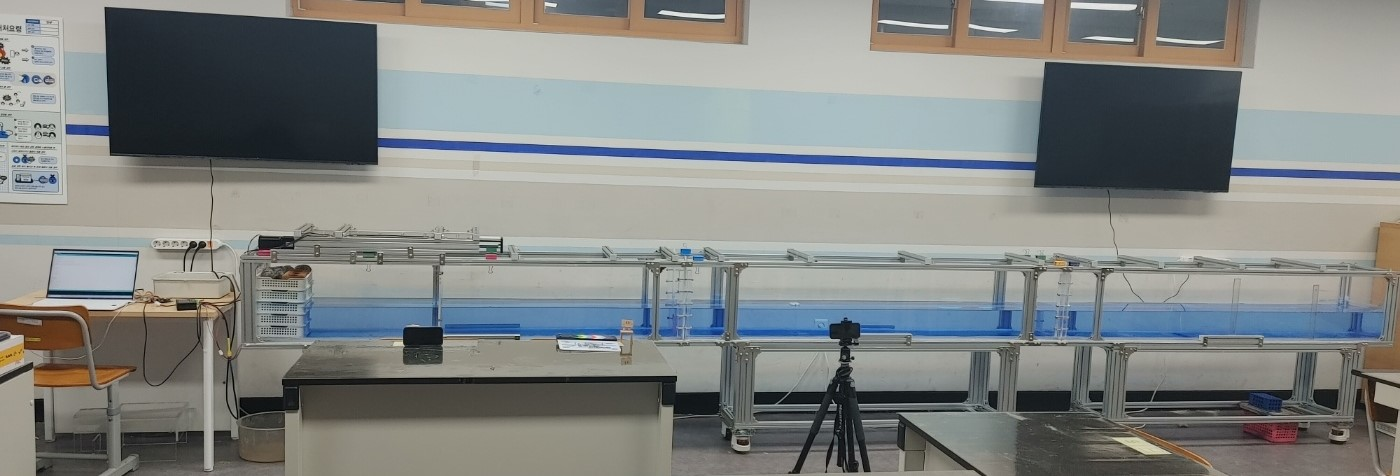
\includegraphics[width=\textwidth]{images/Experiment_System_Crop}
        \captionof{figure}{완성된 조파수조의 모습}
        
 %       \label{Experimnet_System} 
        \begin{tikzpicture} [remember picture, overlay, anchor=north west]
            \node [draw=yellow, text=yellow] (TV1) at (2.5, 5.8) {\scriptsize{TV1}};
            \node [draw=yellow, text=yellow] (TV2) at (14, 5.5) {\scriptsize{TV2}};
            \node [draw=yellow, text=yellow] (computer) at (1.0, 4) {\scriptsize{computer}};
            \node [draw=yellow, text=yellow] at (4.6, 2.6) {\scriptsize{camera1}};
            \node [draw=yellow, text=yellow] at (9.5, 2.5) {\scriptsize{camera2}}; 
        \end{tikzpicture}
        %\captionof{figure}{\scriptsize 완성된 조파 수조의 모습} %\\[0.5em]\
\end{figure}
 
제작한 작품은 '2차원 조파 수조'로 명명하였다. 이 조파 수조를 이용하여 실험을 할때 제대로 진행이 되려면 조파기, 소파기, 파고계, 해안 경사로 등이 제 역할을 해 주어야 가능하다. 따라서 각 부분은 실험 목적에 따라 조립과 분해가 가능하도록 따로 제작하였다. 제작한 조파 수조의 특징을 나열하면 다음과 같다.

\begin{itemize}
    \item 폭 $300~\mathrm{mm}$, 높이 $400~\mathrm{mm}$, 총 길이 $6,000~\mathrm{mm}$의 2차원 조파 수조를 제작하였다. 폭과 높이를 맞추어 수조 모듈을 추가로 제작하여 연결하면 얼마든지 길이를 확장할 수 있다. 
    \item 조파기는 리니어 엑츄레이터를 이용하여 구동부를 제작하였고 틴지 보드를 기반으로 하여 스텝 모터를 움직이는 제어부를 제작하였다. 
    \item 현재 조파기로 규칙파를 생성하는 코드를 완성하여 검증하고 있으며, 코드가 정교화되면 원하는 주기, 파장, 파고의 규칙파를 생성할 수 있다. 
    \item 이후 조파기는 쓰나미 등의 불규칙파를 생성할 수 있도록 정교한 제어를 할 수 있도록 코드를 업그레이드 할 예정이다. 
    \item 해안 경사로는 교각 위에 아크릴 판을 올리는 구조로 설계하여 길이와 기울기를 변화시켜 탈부착이 가능하도록 제작하였다. 
    \item 파고계는 물에 잘 뜨는 재질로 제작하여 동영상 분석을 통해 파고를 파악하고 있으며, 이후 센서를 부착하여 정밀한 파고를 측정하도록 개선할 예정이다.
\end{itemize}

\subsection{수조 모듈 구성 및 연결 방법}
수조는 길이 $2,000~\mathrm{mm}$, 폭 $300~\mathrm{mm}$, 높이 $400~\mathrm{mm}$인 수조 모듈로 구성되어 있으며 3개를 연결하여 총 길이 $6,000~\mathrm{mm}$이다. 수조 모듈의 기본 프레임은 알루미늄 프로파일로 제작하였으며 그 안에 두께 $5~\mathrm{mm}$의 아크릴 판을 이용하여 물이 담기는 수조를 제작하였다. 수조의 모서리 부분은 인접한 두 아크릴 판을 아크릴 접착제로 붙였으며 추가적으로 실리콘으로 방수 처리를 하였다. $2,000~\mathrm{mm}$ 길이의 수조 모듈을 서로 연결할 때는 물이 새지 않도록 매우 정교하게 붙여야 한다. 특히, 수준기로 수평이 맞는지 여러 방향에서 확인하여 모듈 3개가 일직선을 이루도록 해야 한다. 수조 모듈을 연결하는 연결부는 실리콘 패드를 잘라 모듈 사이에 끼웠고 아크릴 판의 옆, 아래에는 볼트가 들어갈만한 크기의 아크릴 조인트를 부착하여 볼트와 너트로 조이는 방법을 채택하였다. 수조 연결부도 실리콘으로 방수 처리를 하여 물이 새지 않는 총 길이 $6,000~\mathrm{mm}$의 수조를 완성하였다. 더 긴 수조가 필요하면 규격에 맞는 수조 모듈을 추가로 제작하여 사이에 끼워 붙여 길게 확장이이 가능하다.

\begin{figure}[h]
	\begin{center}
		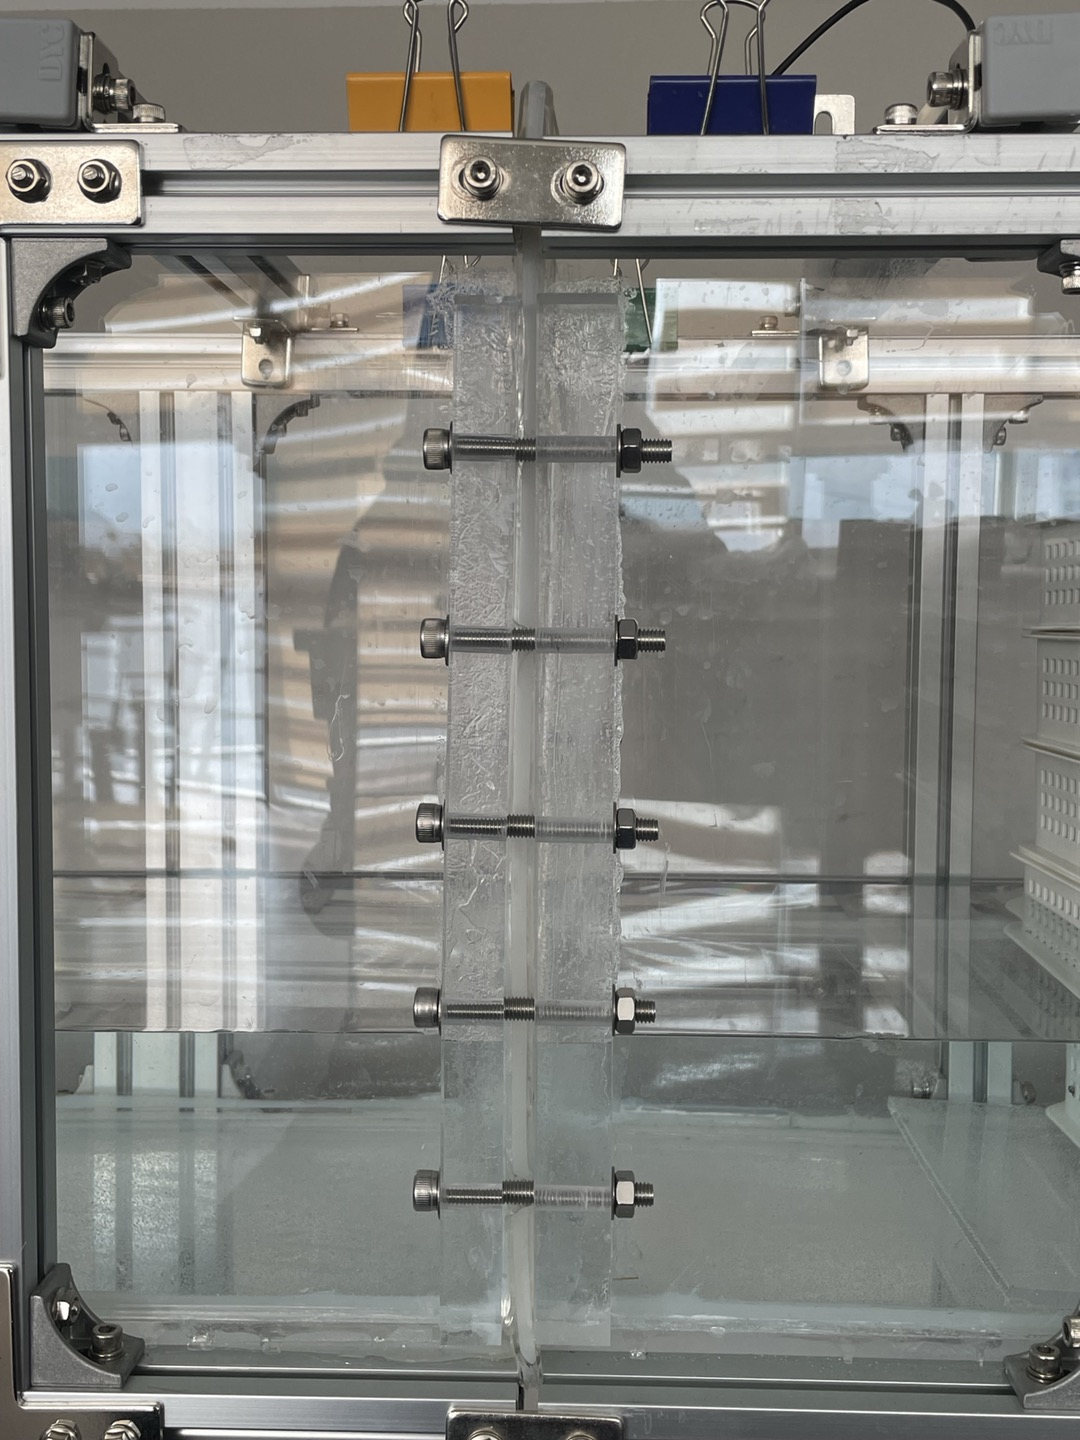
\includegraphics[width=0.3\textwidth]{images/magam1.jpg}
		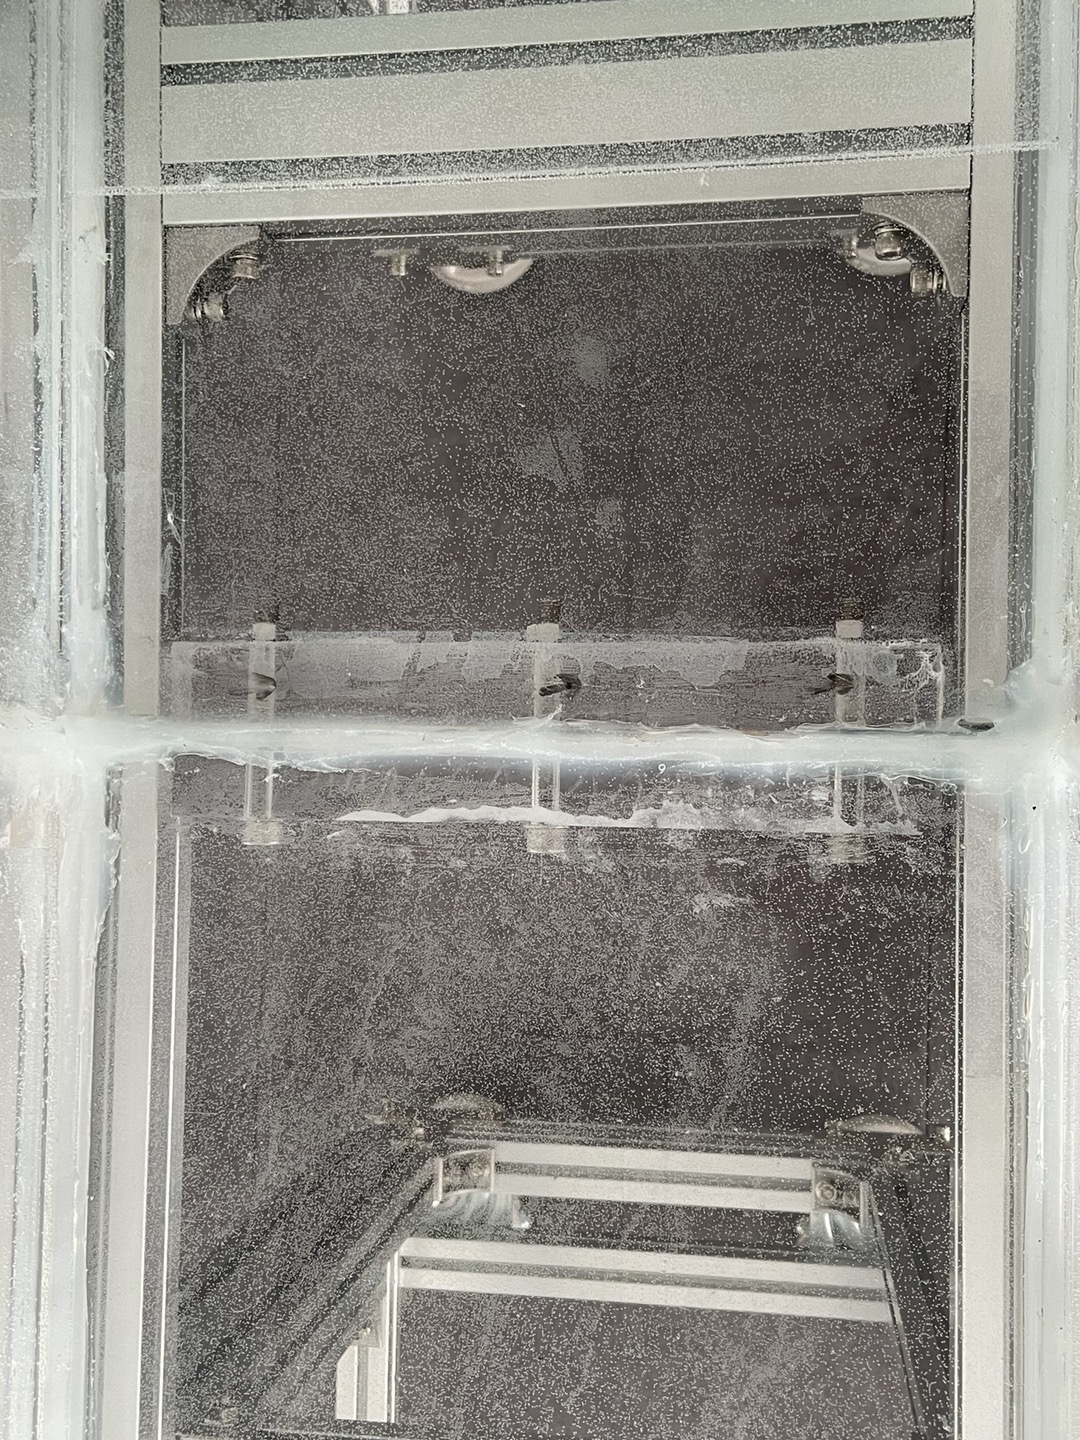
\includegraphics[width=0.3\textwidth]{images/magam2.jpg}
		\caption{수조 연결부의 모습}
		\label{Waveabsorber}
	\end{center}
\end{figure}

\subsection{소파 장치}
해파가 전파되다가 벽이나 장애물에 부딫히게 되면 반사파가 발생하는데, 수조는 양 끝이 막힌 구조로 되어 있어 조파기에서 출발한 해파와 반사파가 간섭을 일으키고 결과적으로 정상파가 만들어져 해파 실험에 지장을 준다. 대부분의 실험에서는 맞춤형 환경 조성을 위해 반사파를 상쇄시키는 소파 장치가 매우 중요하다.

조파판이 식 (\ref{eq:7})\을 따라 움직이면서 판의 뒷부분으로 진행하는 파도 생성한다. 판의 앞부분으로 진행하는 파는 수조의 말단에서 정상파를 형성하지만 $x/h > 20$이므로 (수심은 채 $30\mathrm{~cm}$가 되지 않는다.) 충분히 무시할 수 있다. 하지만 이는 수조가 무한히 길다고 가정한 상황이며 우리 수조의 경우 비록 $x/h > 20$이지만 반사파가 생길 수 있다. 또, 판의 뒷부분으로 진행하는 파는 상당히 좁은 공간에서 계속 중첩되므로 판에 계속해서 부하를 가하기 때문에 파를 소멸시킬 소파 장치가 필요하다.

\begin{figure}[h]
	\begin{center}
		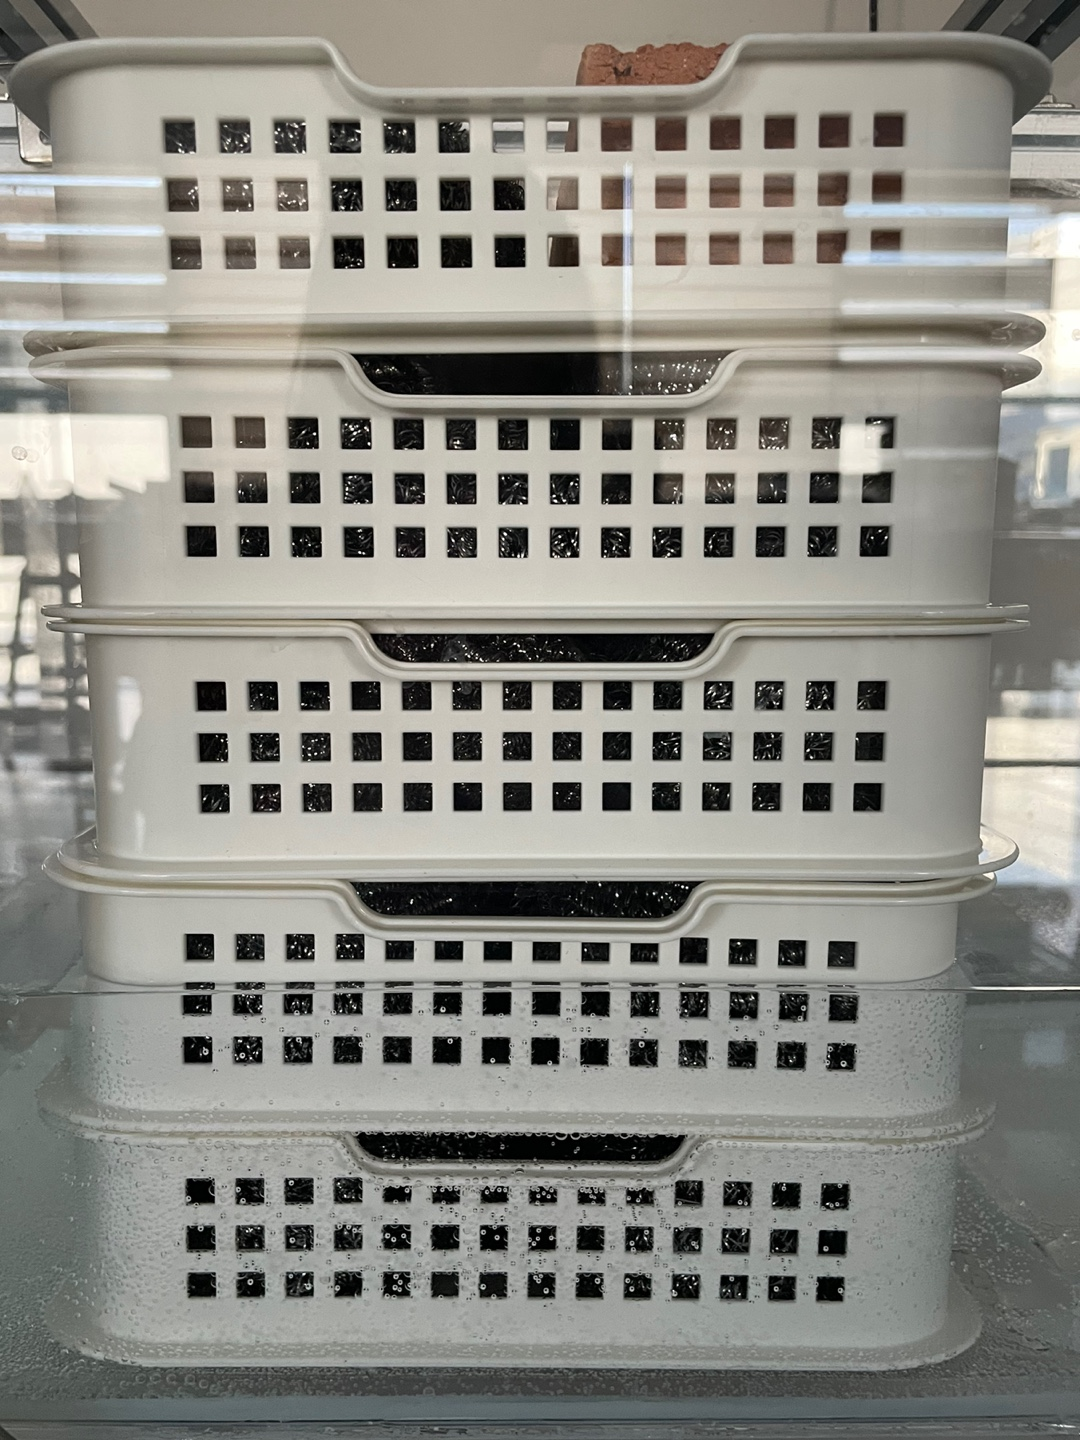
\includegraphics[width=0.3\textwidth]{images/sopagi1.jpg}
		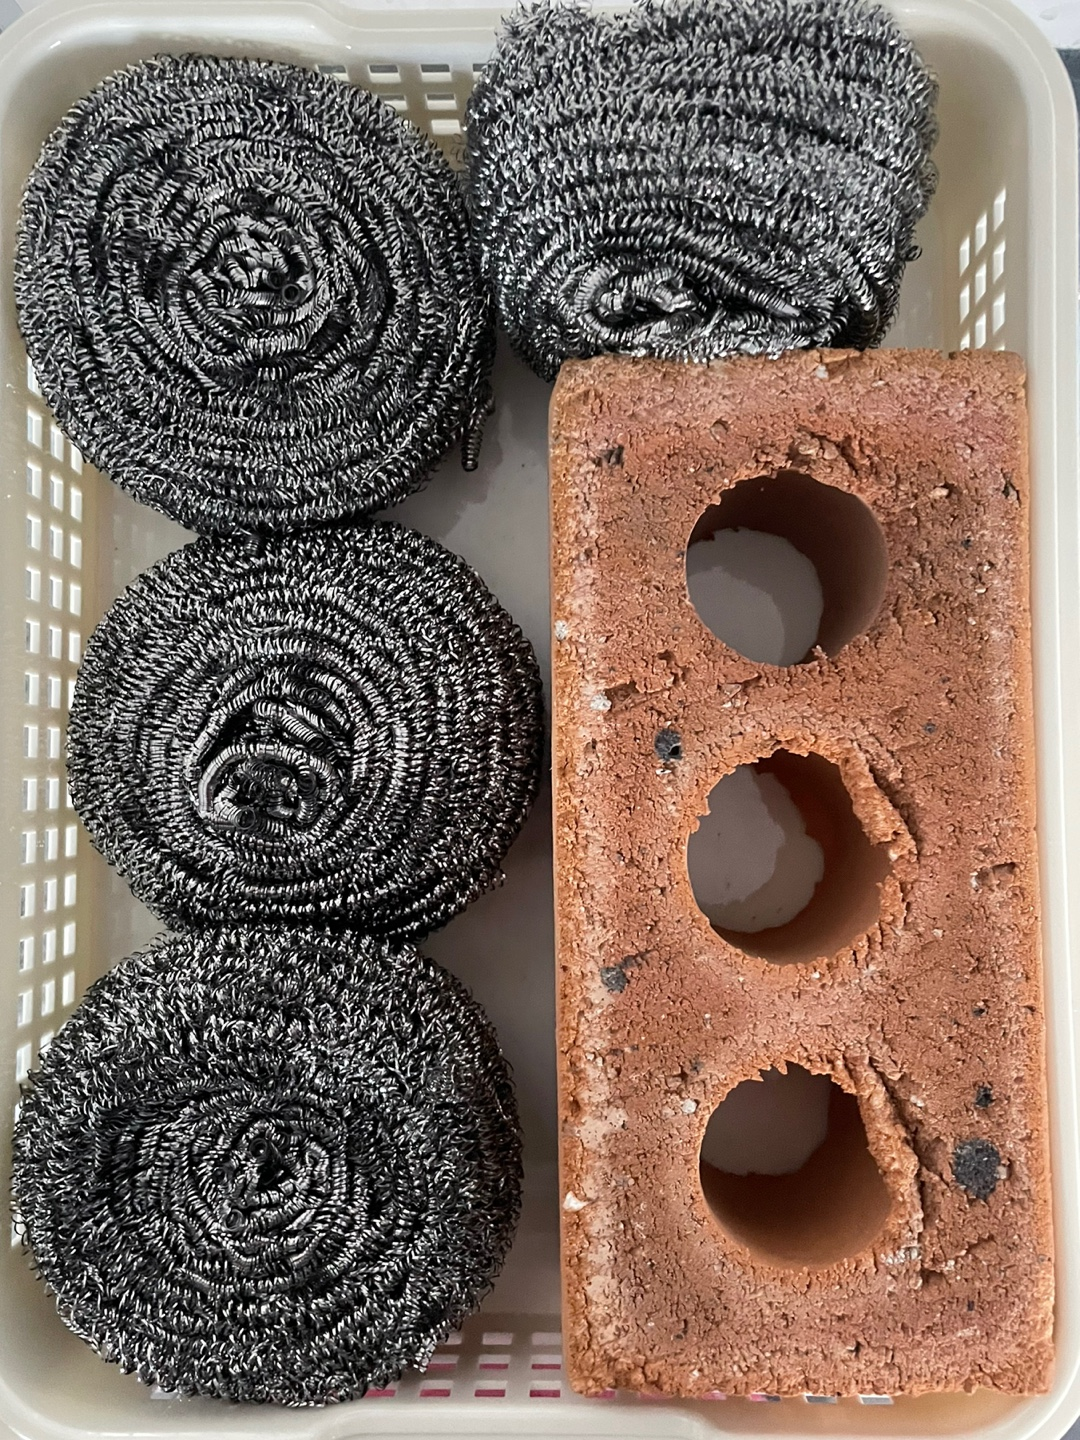
\includegraphics[width=0.3\textwidth]{images/sopagi2.jpg}
		\caption{플라스틱 바구니와 수세미를 이용해 만든 소파 장치}
		\label{Waveabsorber}
	\end{center}
\end{figure}

소파 장치는 해파의 에너지를 흡수할 수 있는 다공질의 구조가 소파 성능이 좋다는 점에 착안하여 구멍이 뚫린 플라스틱 바구니에 철 수세미를 넣는 방식으로 간단하게 제작하였다 \cite{lim2014optimum, o2017methods}. 플라스틱 바구니에 철수세미를 최대한 밀착하여 집어넣어 다공성 구조를 형성해주었고 소파 장치가 가벼워 파도에 의해 움직이기 때문에 이를 고정시키기 위해 가장 윗 칸에 벽돌을 올려 눌러주었다. 이렇게 2개를 만들어 조파 수조의 양 말단에 설치할 수 있도록 하였다. 

\subsection{연안 모형(해안 경사)}

먼 바다에서 해안으로 올수록 수심이 얕아지므로 해파는 심해파, 천이파, 천해파로 바뀌면서 바닥의 영향을 많이 받게 된다. 이 과정에서 파가 굴절하기도 하고, 속도가 느려지면서 쇄파 현상이 발생하게 된다. 해파는 연안의 모양에 따라 서로 다른 영향을 줄 수 있어 여러 연안 모형에 대해서 실험을 해야할 경우가 존재한다.

이러한 점을 감안하여 연안 모형은 목적에 맡게 바꿀 수 있고 탈부착이 가능하도록 설계하였다. 일정한 너비의 아크릴 판을 수조 바닥에 부착하고 육지 쪽은 높이 차를 만들기 위해 해안 경사 바닥을 안정적으로 지지할 수 있도록 알루미늄 프로파일 교각을 설치하였다. 실제 우리나라 주변의 바다만 하더라도 동해, 황해, 남해의 전형적인 해안 경사가 다르고, 해안 경사는 해파의 영향으로 항상 변할수 있기에 다양한 기울기의 해안 경사를 가질 수 있도록 해안 경사 바닥을 지지하는 교각의 길이를 다양하게 준비해 두었다. 현재 설치한 경사로는 높이 $200\mathrm{~mm}$, 길이 $2,000\mathrm{~mm}$로 기울기가 $1/10$ 이다. 

\begin{figure}[htbp]
	\begin{center}
		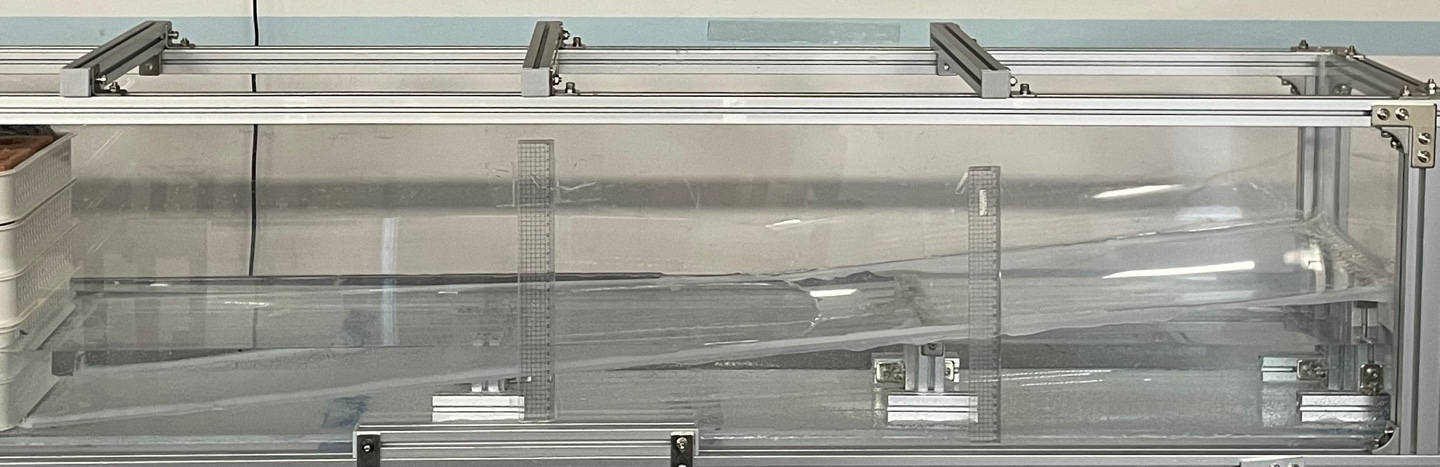
\includegraphics[width=0.8\textwidth]{images/slope.jpg}
		\caption{설치한 연안 모형}
		\label{Slope}
	\end{center}
\end{figure}


\subsection{방파제 모형}
현재 해안 모형은 경사로로 두었다. 하지만 경사로를 앞으로 이동시키고 뒷부분의 공간에 평지를 두면 구조물을 설치할 수 있다. 여기에 파력 발전 시설을 두어 여러 발전 시스템의 효율 비교 및 최적화 연구를 진행할 수도 있고 구조물의 내구성 실험을 할 수도 있다. 나아가 경사로의 경사로 변화시켜 여러 환경에서 다양한 실험을 진행할 수 있다. 또, 경사로를 받치는 부품이 녹슬었는데 이는 다른 재료로 대체하거나 경사로를 판을 덧대는 것이 아닌 일체형으로 만들어 관리가 쉽게 할 예정이다.

\begin{figure}[htbp]
    \centering
    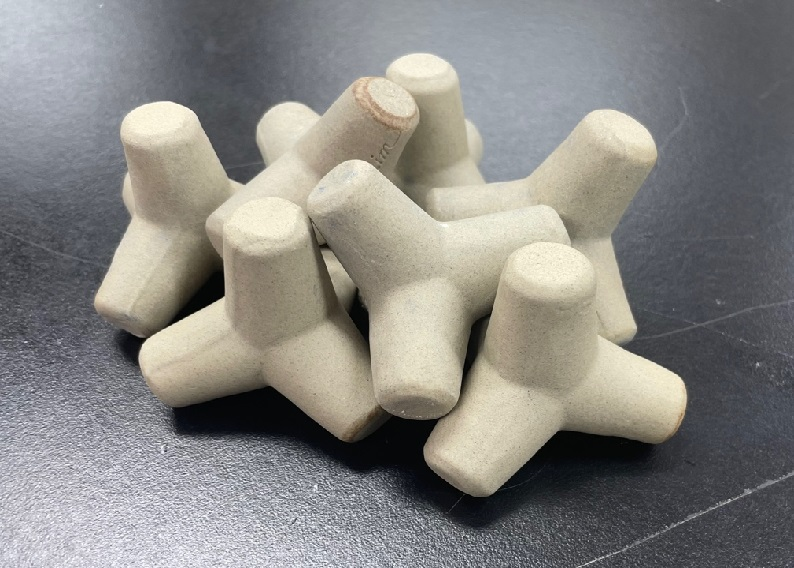
\includegraphics[height=5.5cm]{images/Breakwater.jpg}
    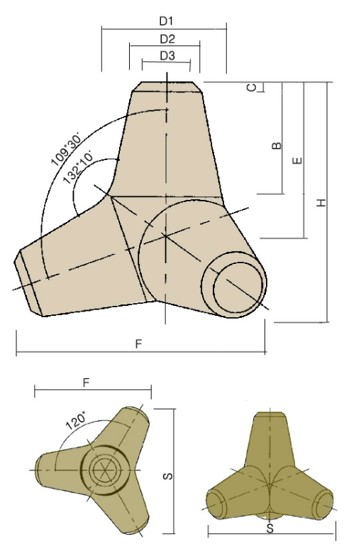
\includegraphics[height=5.5cm]{images/Breakwater(Illustrated).jpg}
    \caption{방파제 모형(왼쪽)과 규격(오른쪽)}
    \label{Braekwater}
\end{figure}

규격 $D3=1.2\mathrm{~cm}, D2=1.7\mathrm{~cm}, S=5.3\mathrm{~cm}, F=5\mathrm{~cm}$의 방파제 모형을 이용한 연구를 진행할 예정이다. 방파제의 조적 구조는 Gurer의 구조, Fabiao의 구조 등 여러 종류가 있으며 구조의 종류 및 스케일에 대한 방파 효과를 비교할 수도 있다\cite{article}.




\subsection{조파기}

%조파기 설계도를 넣어야 하는가? (넣는다면 다시 그릴 필요가 있음. 이전에 그렸던 것은 비율도 맞지 않고 전체적인 모습을 나타내지 못 함)

%조파기 사진
조파기는 구동부와 제어부로 나뉜다. 구동부는 조파기의 기계적인 부분으로 실질적인 움직임을 담당하며 리니어 액츄에이터와 이를 고정할 여러 부품으로 구성되어 있다. 제어부는 모터의 회전을 제어하는 부분으로 모터 드라이버와 틴지 보드 3.2(Teensy Board)로 구성되어 있다.

\subsubsection{구동부}
구동부는 $80\mathrm{~cm}$ 길이의 리니어 액츄에이터(linear actuator)를 메인 부품으로 하여 알루미늄 프로파일 프레임을 만들었다. 리니어 액츄에이터의 운동부에는 아크릴 재질의 조파판을 달았다. 조파판이 조파 수조 내부에 들어가도록 구동부를 수조 위에 설치하였다. 아크릴 판이 조파판이며 규격은 $280\mathrm{~mm} ~\times~ 295\mathrm{~mm} ~\times~5\mathrm{~mm}$로 수조 내부 공간에 딱 들어맞게 제작하였다. 조파판이 수조 내부의 벽과 최대한 밀착되어 있어야 정교한 파를 생성할 수 있다. 리니어 액츄에이터의 이동부에 붙어 수조 내부를 수평적으로 이동하며 물을 밀어내고 파를 생성한다. 액츄에이터는 FUYU 사의 FSK80 시리즈 제품으로 가동범위(stroke)는 $80\mathrm{~cm}$이고 최대 힘 $40\mathrm{~N}$, 최대 속력 $23\mathrm{~cm/s}$을 낼 수 있다(표 \ref{Specification of Linear Actuator}).

% \begin{figure}[H]
%     \begin{minipage}[t]{.3\linewidth}
%     \begin{center}
%         \scalebox{-1}[1]{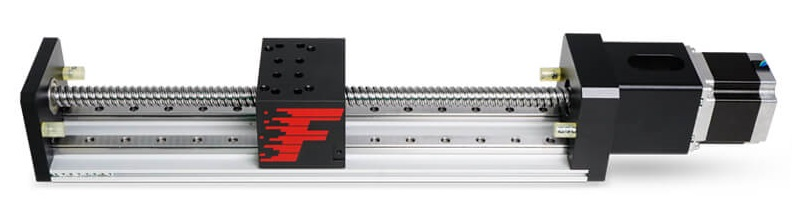
\includegraphics[width = 3cm]{images/Linear_Actuator.jpg}}
%         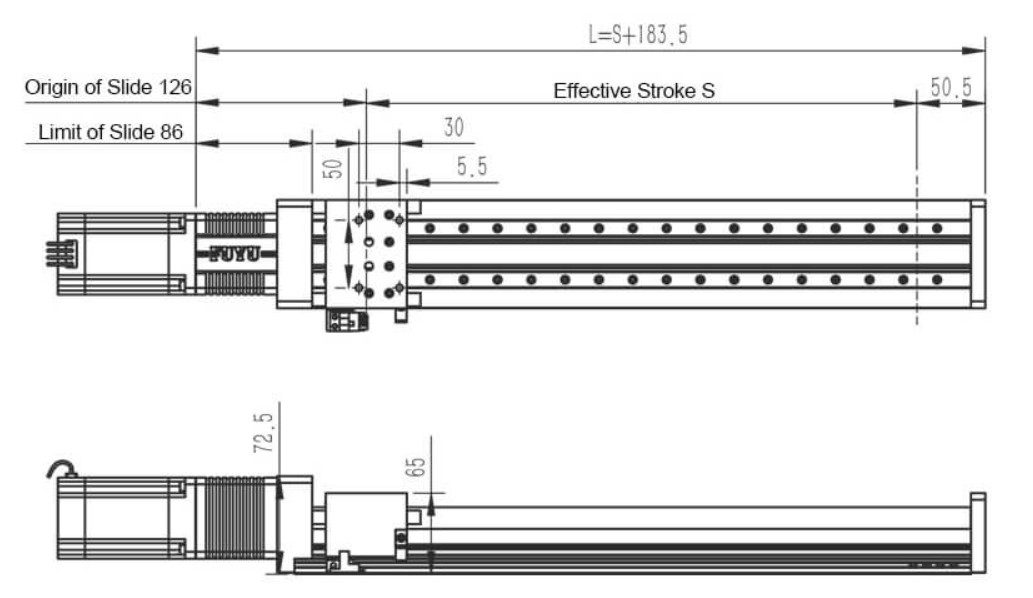
\includegraphics[width = 3cm]{images/Linear_Actuator(Design).jpg}
%     \end{center}
%         \begin{tikzpicture} [remember picture, overlay]
%         \node at (2.0, 11.0) {(a)};
%         \node at (2.0, 7.6) {(b)}; %1.1
%         \end{tikzpicture}	
%         %\caption{Linear actuator - (a) \textit{FSK80} series (b) Design}
%         \caption{(a) FUYU사의 FSK80 시리즈 리니어 액츄에이터, (b) 제원}
%         \label{linear actuator}
%     \centering
%   \end{minipage}\hfill
  
%   \begin{minipage}[t]{.6\linewidth}
%     \centering
%     \captionsetup{justification=centering}
%     \caption{리니어 액츄에이터의 스펙}
%     \begin{tabular}{l|l}
%         \hline
%         guide width $(\mathrm{mm})$                       & 80                                     \\
%         repeat position accuracy $(\mathrm{mm})$          & $\pm$0.02                                 \\
%         motor                                  & stepper 60102                          \\
%         % rail model                             & dual rail W12 $\times$ H8              \\
%         % ball screw model                       & 16                                     \\
%         \textbf{stroke $(\mathrm{mm})$}                  & \textbf{50 - 1000}                                    \\
%         pitch                                  & 10                                     \\
%         \textbf{horizontal full payload speed $(\mathrm{mm/s})$}   & \textbf{230}                                    \\
%         vertical full payload speed $(\mathrm{mm/s})$     & 60                                     \\
%         side mounting payload speed $(\mathrm{mm/s})$     & 210                                    \\
%         \textbf{rated horizontal payload $(\mathrm{kg})$}          & \textbf{40}                                     \\
%         rated vertical payload $(\mathrm{kg})$            & 20                                     \\
%         rated side mounting payload $(\mathrm{kg})$       & 15                                     \\
%         noisy without payload $(\mathrm{db})$             & 79                                     \\
%         rated payload noisy $(\mathrm{db})$               & 70                                     \\
%         \textbf{acceleration } $(\mathrm{mm/s}^{2})$   & \textbf{500}                                    \\ \hline
%     \end{tabular}%
%     \label{Specification of Linear Actuator}
%   \end{minipage}
% \end{figure}

%%%%%%%%%%%%%%%%%%%%%%%%%%%%%%%%%%%%%%%%%%%%%%%%%%%%%%%%%%%%%%%%%%%%%%%%%%%%%
\begin{figure}[H]
    \begin{center}
        \scalebox{-1}[1]{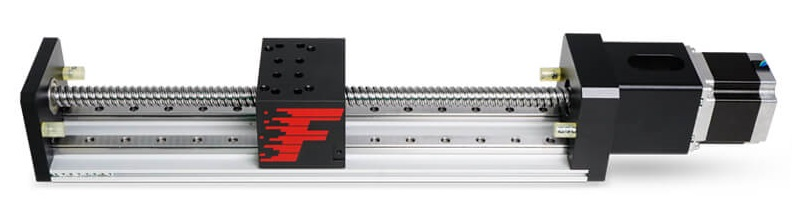
\includegraphics[width = 12cm]{images/Linear_Actuator.jpg}}
        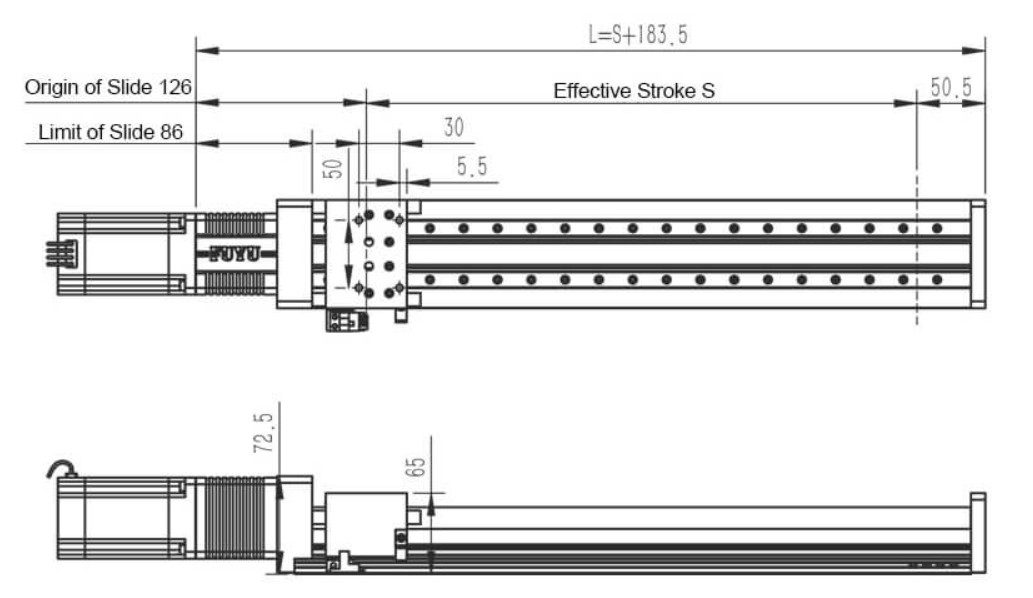
\includegraphics[width = 12cm]{images/Linear_Actuator(Design).jpg}
    \end{center}
        \begin{tikzpicture} [remember picture, overlay]
        \node at (2.0, 11.0) {(a)};
        \node at (2.0, 7.6) {(b)}; %1.1
        \end{tikzpicture}	
        %\caption{Linear actuator - (a) \textit{FSK80} series (b) Design}
        \caption{(a) FUYU사의 FSK80 시리즈 리니어 액츄에이터, (b) 제원}
        \label{linear actuator}
\end{figure}
%%%%%%%%%%%%%%%%%%%%%%%%%%%%%%%%%%%%%%%%%%%%%%%%%%%%%%%%%%%%%%%%%%%%%%%%%%%%

% \begin{figure}[H]
%     \centering
%     \captionsetup{justification=centering}
%     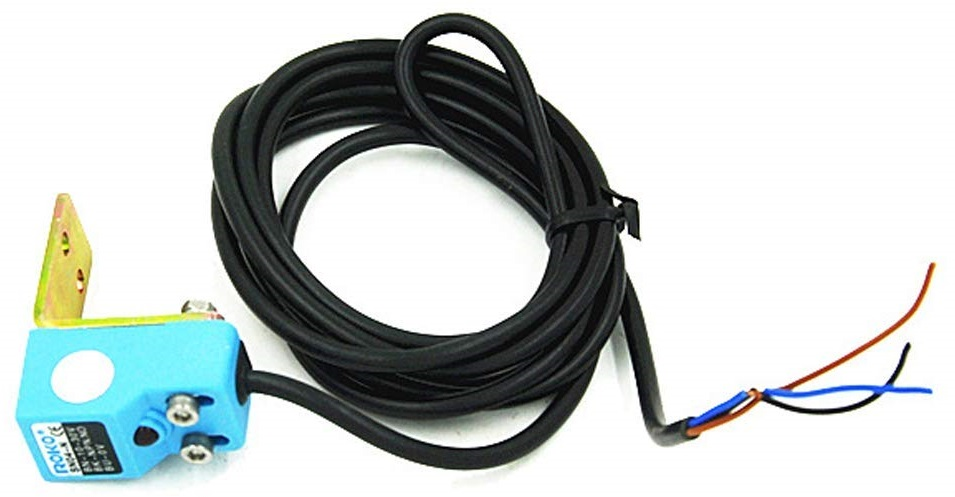
\includegraphics[width = 6cm]{images/Limit_Switch.jpg}
%     \caption{Limit Switch}
%     \label{limit switch}
% \end{figure}

% \begin{figure}
%     \centering
%     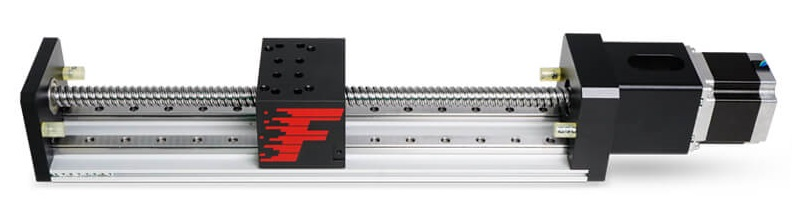
\includegraphics[width=0.5\textwidth]{images/Linear_Actuator.jpg}
%     \caption{FUYU사의 FSK80 시리즈 리니어 액츄에이터}
%     \label{Linear Actuator}
% \end{figure}

\begin{figure}
    \begin{minipage}[b]{.45\linewidth}
        \centering
        \scalebox{-1}[1]{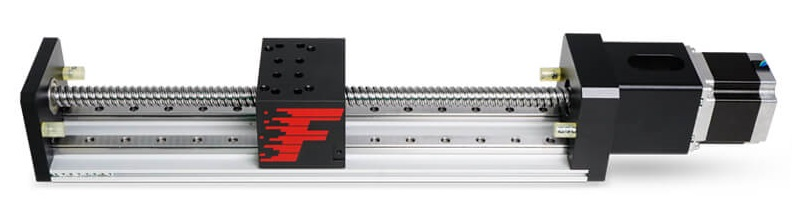
\includegraphics[width = 0.45\linewidth]{images/Linear_Actuator.jpg}}
        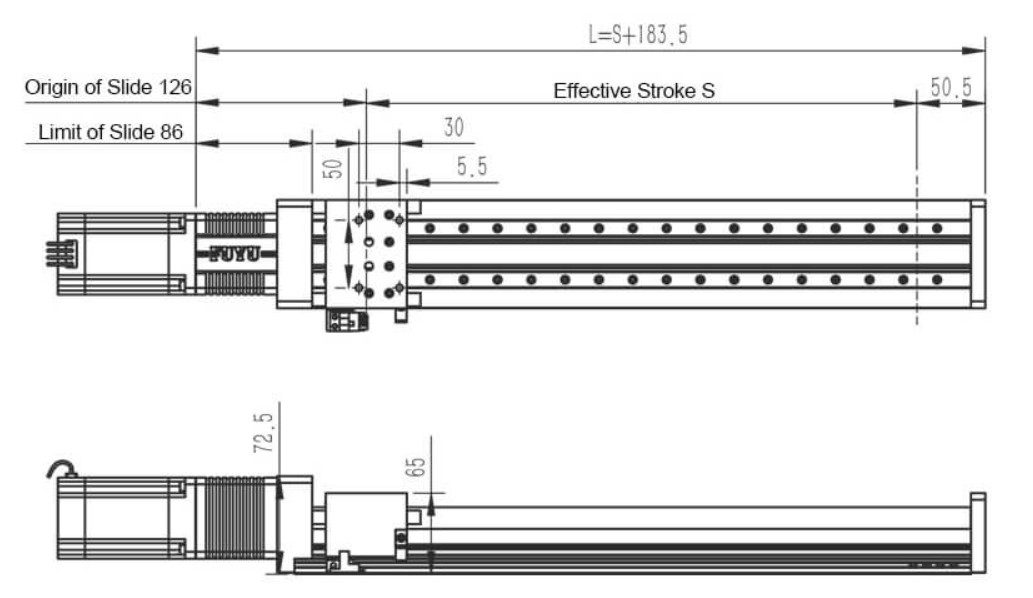
\includegraphics[width = 6cm]{images/Linear_Actuator(Design).jpg}
        % \begin{tikzpicture} [remember picture, overlay]
        %     \node at (2.0, 11.0) {(a)};
        %     \node at (2.0, 7.6) {(b)}; %1.1
        % \end{tikzpicture}	
        %\caption{Linear actuator - (a) \textit{FSK80} series (b) Design}
        \captionof{figure}{FUYU사의 FSK80 시리즈 리니어 액츄에이터}
        \label{linear actuator}
    \end{minipage}\hfill
    
    \begin{minipage}[b]{.45\linewidth}
        \resizebox{\columnwidth}{!}{
        \begin{tabular}{l|l}
            \hline
            guide width $(\mathrm{mm})$                       & 80                                     \\
            repeat position accuracy $(\mathrm{mm})$          & $\pm$0.02                                 \\
            motor                                  & stepper 60102                          \\
            % rail model                             & dual rail W12 $\times$ H8              \\
            % ball screw model                       & 16                                     \\
            \textbf{stroke $(\mathrm{mm})$}                  & \textbf{50 - 1000}                                    \\
            pitch                                  & 10                                     \\
            \textbf{horizontal full payload speed $(\mathrm{mm/s})$}   & \textbf{230}                                    \\
            vertical full payload speed $(\mathrm{mm/s})$     & 60                                     \\
            side mounting payload speed $(\mathrm{mm/s})$     & 210                                    \\
            \textbf{rated horizontal payload $(\mathrm{kg})$}          & \textbf{40}                                     \\
            rated vertical payload $(\mathrm{kg})$            & 20                                     \\
            rated side mounting payload $(\mathrm{kg})$       & 15                                     \\
            noisy without payload $(\mathrm{db})$             & 79                                     \\
            rated payload noisy $(\mathrm{db})$               & 70                                     \\
            \textbf{acceleration } $(\mathrm{mm/s}^{2})$   & \textbf{500}                                    \\ \hline
        \end{tabular}}%
        \captionof{table}{스펙}
        \label{Specification of Linear Actuator}
    \end{minipage}
\end{figure}


\begin{table}[H]
    \centering
    \captionsetup{justification=centering}
    \caption{리니어 액츄에이터의 스펙}
    \begin{tabular}{l|l}
        \hline
        guide width $(\mathrm{mm})$                       & 80                                     \\
        repeat position accuracy $(\mathrm{mm})$          & $\pm$0.02                                 \\
        motor                                  & stepper 60102                          \\
        % rail model                             & dual rail W12 $\times$ H8              \\
        % ball screw model                       & 16                                     \\
        \textbf{stroke $(\mathrm{mm})$}                  & \textbf{50 - 1000}                                    \\
        pitch                                  & 10                                     \\
        \textbf{horizontal full payload speed $(\mathrm{mm/s})$}   & \textbf{230}                                    \\
        vertical full payload speed $(\mathrm{mm/s})$     & 60                                     \\
        side mounting payload speed $(\mathrm{mm/s})$     & 210                                    \\
        \textbf{rated horizontal payload $(\mathrm{kg})$}          & \textbf{40}                                     \\
        rated vertical payload $(\mathrm{kg})$            & 20                                     \\
        rated side mounting payload $(\mathrm{kg})$       & 15                                     \\
        noisy without payload $(\mathrm{db})$             & 79                                     \\
        rated payload noisy $(\mathrm{db})$               & 70                                     \\
        \textbf{acceleration } $(\mathrm{mm/s}^{2})$   & \textbf{500}                                    \\ \hline
    \end{tabular}%
    \label{Specification of Linear Actuator}
\end{table}


\begin{figure}[H]
    \centering
        \includegraphics[width=0.8\textwidth]{images/jopagi.jpg} 
    \caption{피스톤형 조파기의 구동부 모습}
    \label{wavemaker-photo}
\end{figure}
%%%%%%%%%%%%%%%%%%%%%%%%%%%%%%%%%%%%%%%%%%%%%%%%%%%%%%%%%%%%%%%%%%%%%%%%%

% \begin{figure}[H]
% 	\begin{center}
% 		\includegraphics[width=.7\textwidth]{jopagi.jpg}
% 		\caption{완성된 피스톤형 조파기의 모습}
% 		\label{Wavetank}
% 	\end{center}
% \end{figure}

\subsubsection{회로부}

제어부는 틴지 보드 3.2와 DRV8825, Microstep Driver(ST-M5045), $48\mathrm{~V}$ SMPS(Switching Mode Power Supply)로 구성되어 있다. DRV8825와 ST-M5045는 모터 드라이버로 모터의 구동을 제어한다. DRV8825는 pcb 보드에 장착하는 스텝 모터 드라이버이며 ST-M5045 외장형 스텝모터 드라이버이다. SMPS는 변압기로 공급 전압을 높여주는 역할을 하며 36, 48V 변압기로 갈아끼울 수 있다. 틴지 보드 3.2는 메인 CPU 역할을 하며 코드를 실행한다.

\begin{figure}[H]
    \centering
    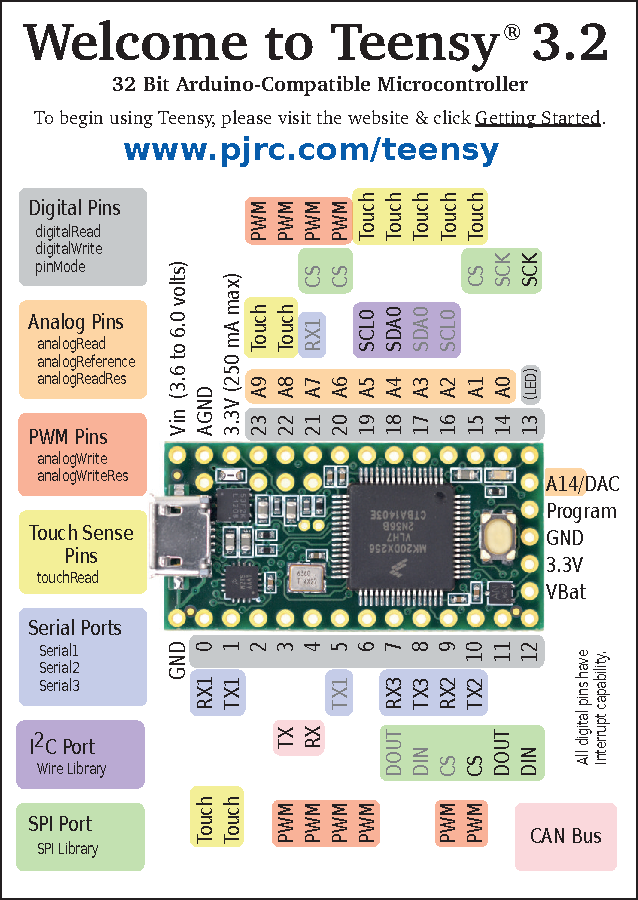
\includegraphics[width=6cm]{images/Teensy3.2 - 1.pdf}
    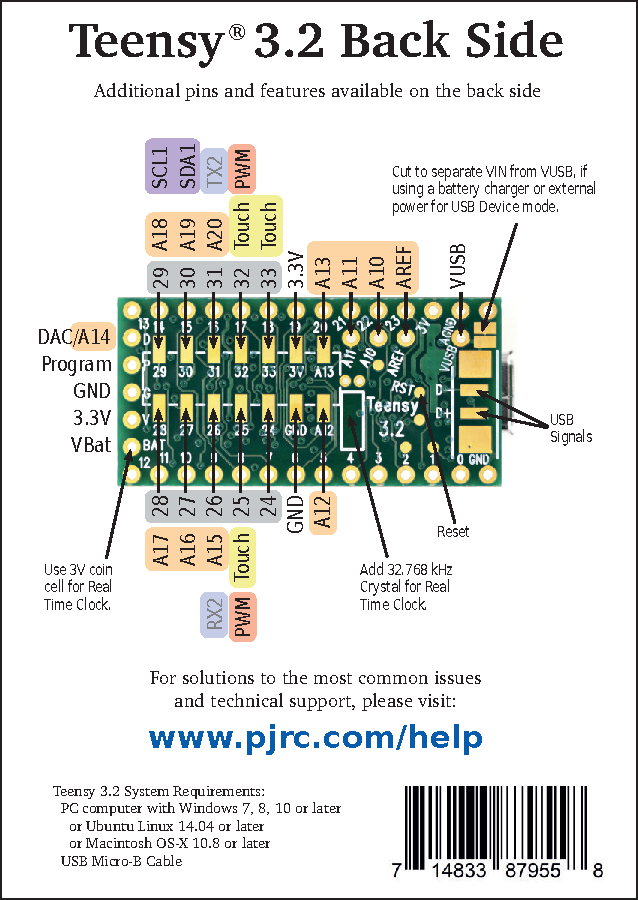
\includegraphics[width=6cm]{images/Teensy3.2 - 2.pdf}
    \caption{틴지 보드의 핀 맵(pin map)}
    \label{fig:enter-label}
\end{figure}


\begin{table}[H]
    \centering
    \caption{틴지 보드의 스펙}
    \begin{tabular}{l}
        \hline
        ARM Cortex-M4 at 72 MHz\\
        256K Flash, 64K RAM, 2K EEPROM\\
        USB device 12 Mbit/sec\\
        34 digital input/output pins, 12 PWM output pins\\
        21 analog input pins, 1 analog output pin, 12 capacitive sense pins\\
        3 serial, 1 SPI, 2 I2C ports\\
        1 I2S/TDM digital audio port\\
        1 CAN bus\\
        16 general purpose DMA channels\\
        RTC for date/time\\
        \hline
    \end{tabular}
    \label{Specification of Teensy Board}
\end{table}



\begin{figure}[H]
	\begin{center}
		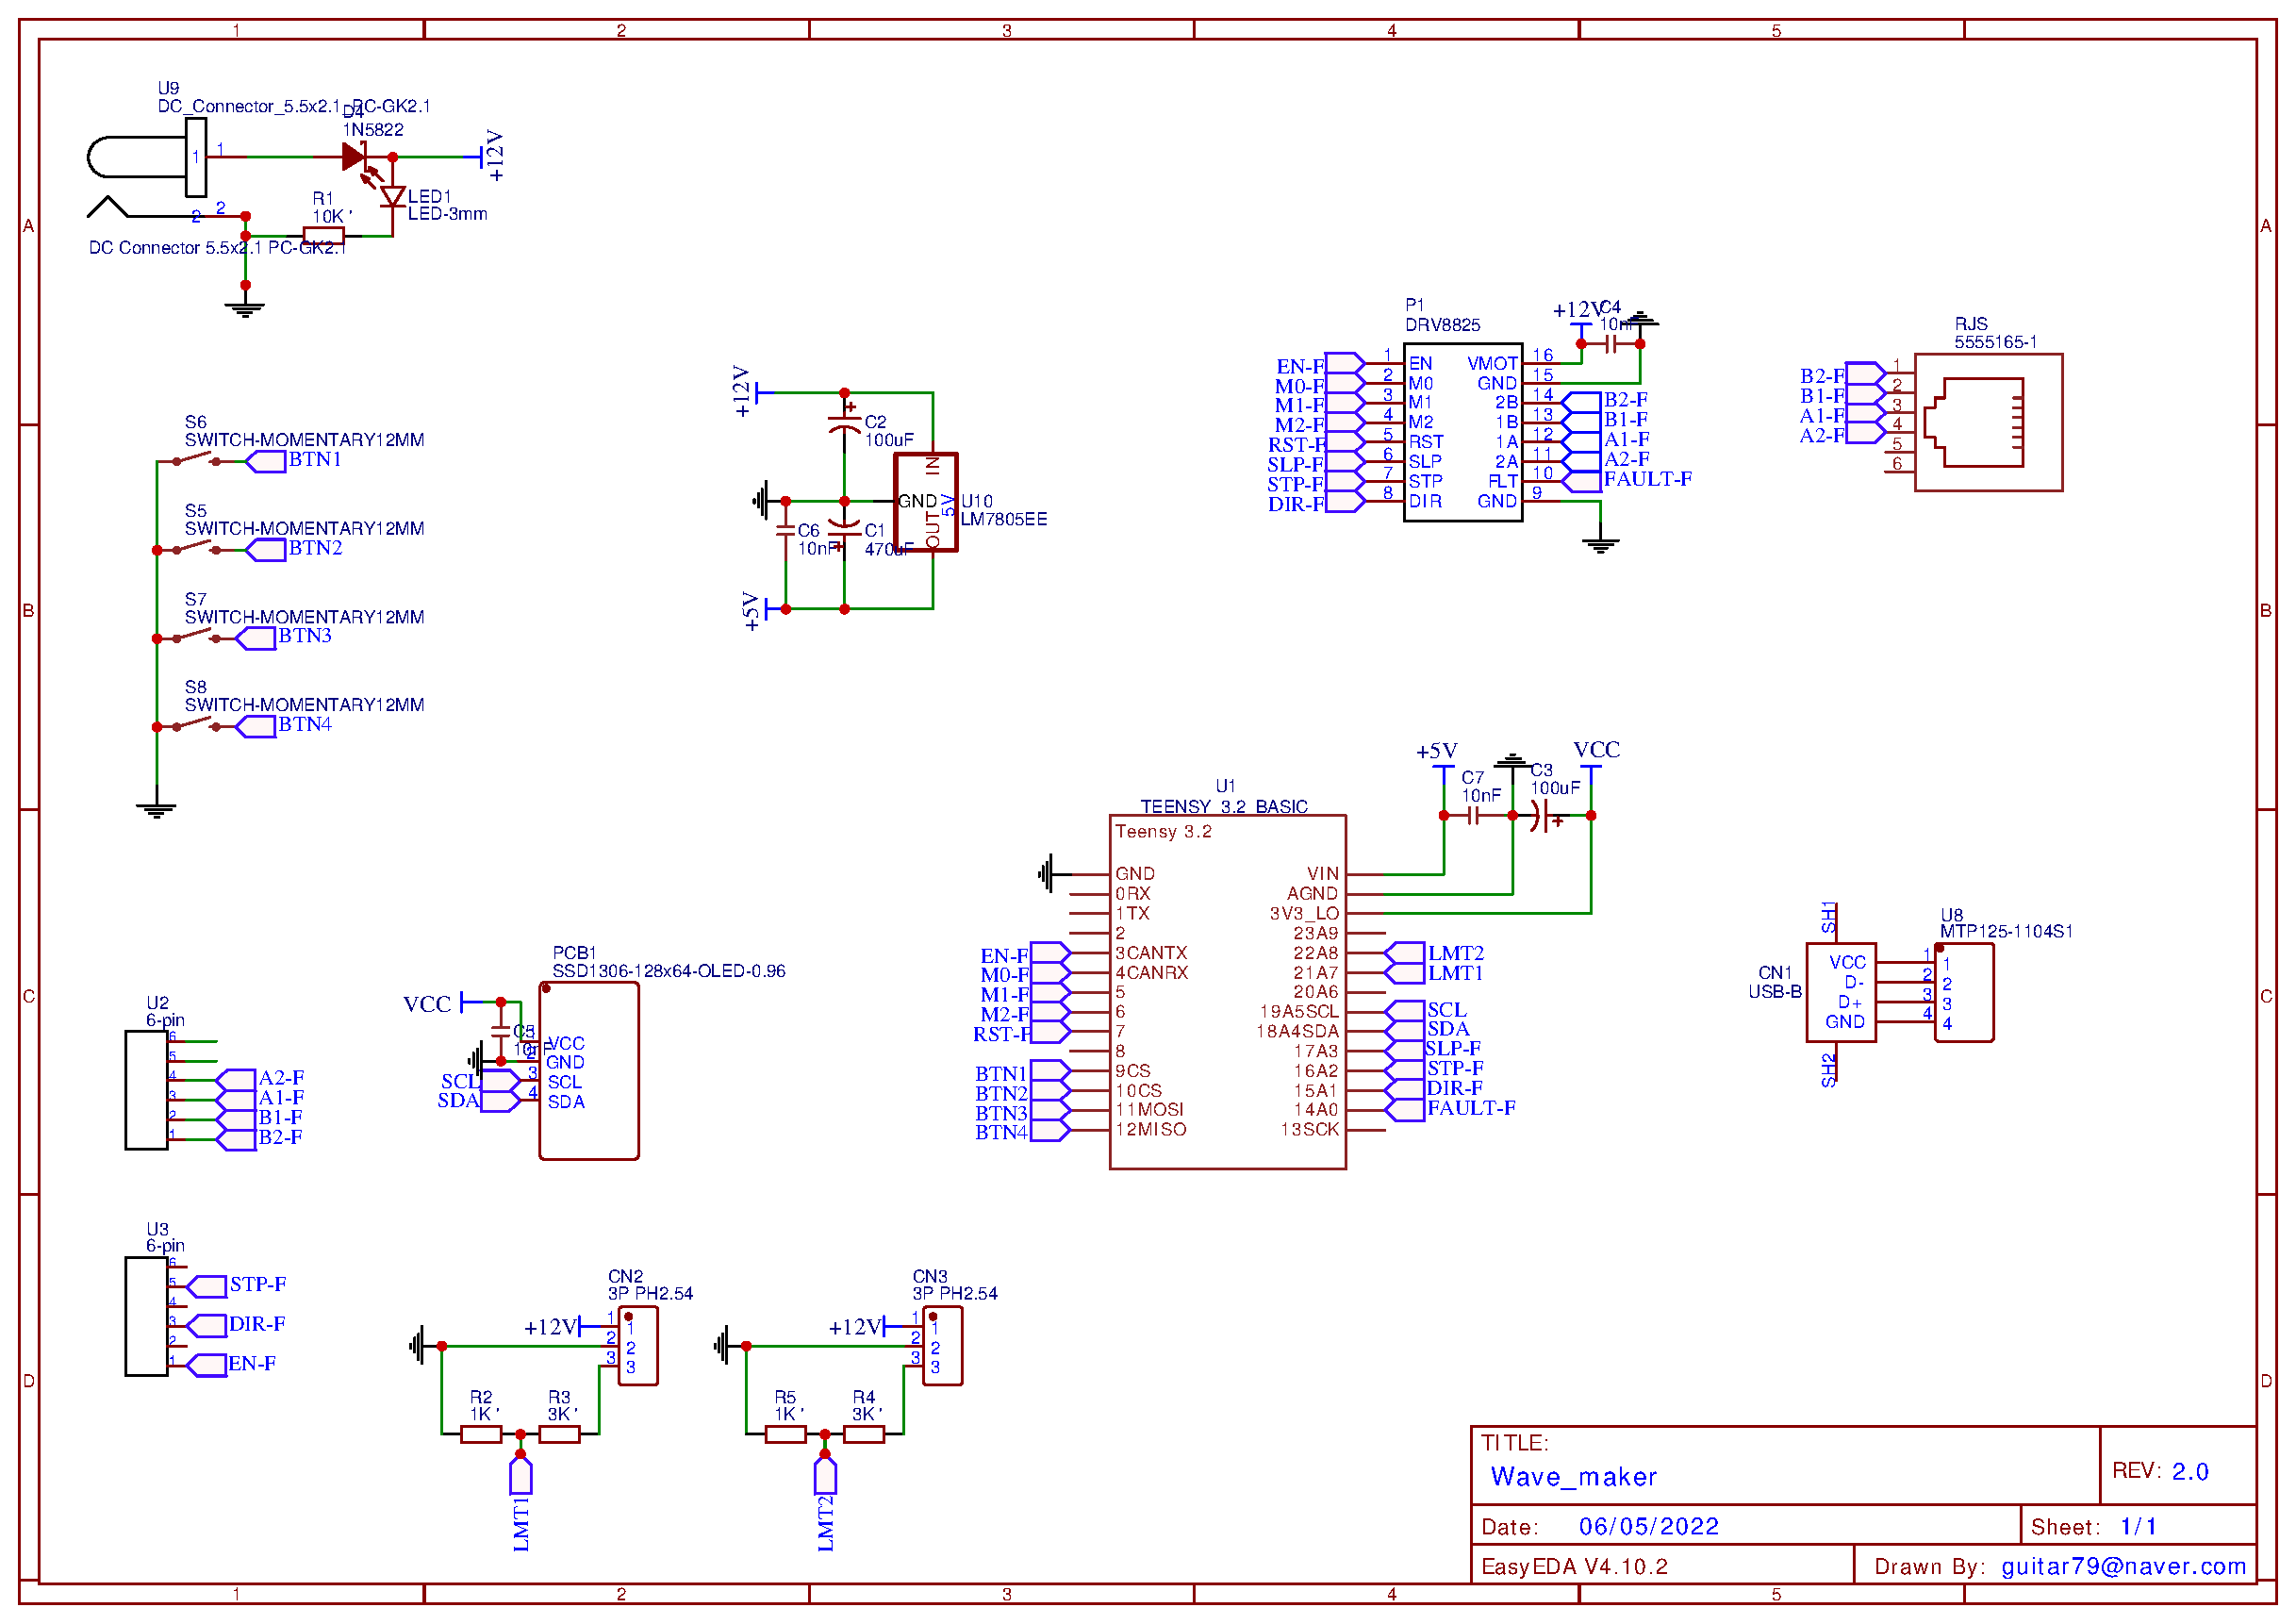
\includegraphics[height=5cm]{Schematic_Wave_maker_2-1_2022-11-24.pdf}
		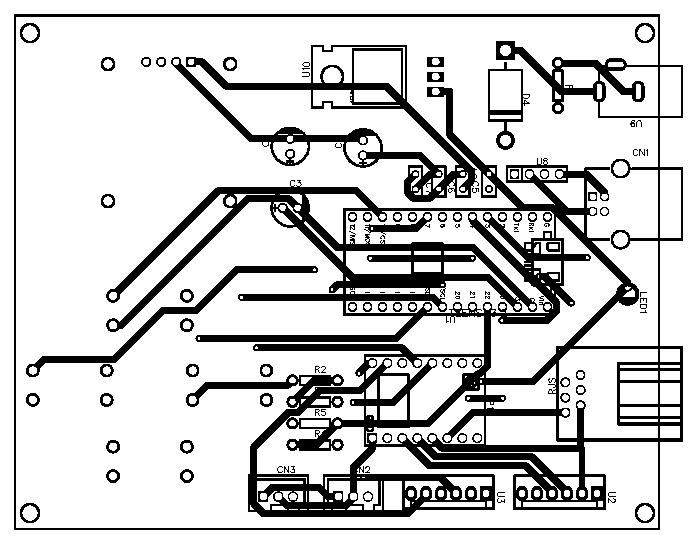
\includegraphics[height=5cm]{PCB_Wave_maker_2022-11-24.pdf}
        \caption{조파기 전자 회로 설계와 제작한 pcb}
		\label{PCB}
	\end{center}
\end{figure}


각 소자를 편리하게 다루기 위하여 pcb를 설계하였다. 틴지 보드 3.2는 3.2$\mathrm{V}$의 구동 전압이 필요하며 상세 스펙은 다음과 같다(표 \ref{Specification of Teensy Board}).



\begin{table}[H]
    \centering
    \caption{조파기 전자 회로에 사용된 부품}
    \label{Specification of Teensy Board}
\begin{tabular}{l|llll}
\hline
ID & Name                             & \multicolumn{2}{l}{Designator}  & Quantity \\ \hline
1  & 10nF                             & \multicolumn{2}{l}{C6,C4,C7,C5} & 4        \\
2  & 470uF                            & \multicolumn{2}{l}{C1}          & 1        \\
3  & 100uF                            & \multicolumn{2}{l}{C2,C3}       & 2        \\
4  & USB-B                            & \multicolumn{2}{l}{CN1}         & 1        \\
5  & 1N5822                           & \multicolumn{2}{l}{D4}          & 1        \\
6  & LED-3mm                          & \multicolumn{2}{l}{LED1}        & 1        \\
7  & DRV8825                          & \multicolumn{2}{l}{P1}          & 1        \\
8  & 10KΩ                             & \multicolumn{2}{l}{R1}          & 1        \\
9  & 5555165-1                        & \multicolumn{2}{l}{RJS}         & 1        \\
10 & TEENSY\_3.2\_BASIC               & \multicolumn{2}{l}{U1}          & 1        \\
11 & 6-pin                            & \multicolumn{2}{l}{U2}          & 1        \\
12 & MTP125-1104S1                    & \multicolumn{2}{l}{U8}          & 1        \\
13 & DC\_Connector\_5.5x2.1\_PC-GK2.1 & \multicolumn{2}{l}{U9}          & 1        \\
14 & LM7805EE                         & \multicolumn{2}{l}{U10}         & 1        \\
15 & SSD1306-128x64-OLED-0.96         & \multicolumn{2}{l}{PCB1}        & 1        \\
16 & Momentary Switch                 & \multicolumn{2}{l}{S1,S2,S3,S4} & 4       
\\ \hline
\end{tabular}
\end{table}


ST-M5045는 리니어 액츄에이터의 모터를 조절하는 모터 드라이버이며 옆의 스위치의 조작에 따라서 스텝 수와 전류 값을 조절하여 외부적으로도 모터 회전의 감도를 바꿀 수 있다.

\begin{table}[H]
    \centering
    \captionsetup{justification=centering}
    \caption{ST-M5045의 스펙}
    \begin{tabular}{ll}
        \hline
        \textbf{DC power input type $(\mathrm{V})$}  & \textbf{24$\sim$50}      \\
        \textbf{Output current $(\mathrm{A})$}       & \textbf{1$\sim$4.5}      \\
        \textbf{Mircostep}           & \textbf{2, 4, 8, 16, 32, 64, 128, 256, 5, 10, 25, 50, 125, 250               }                \\
        Protect form        & Overheated, Short-voltage, over-voltage, over-current protection \\
        Maximum pulse rate $(\mathrm{kHz})$ & 300             \\
        Dimensions               & $120\mathrm{~mm} \times92\mathrm{~mm}\times33\mathrm{~mm}$ \\
        % Weight                   & \textless{}280g \\
        Working environment & Temperature~~-$15\sim40\mathrm{\degree C}$, Humidity~\textless{}$90\%$ \\ 
        \hline
    \end{tabular}
    \label{Specification of ST-M5045}
\end{table}

여러 소자를 연결하여 구성한 조파기의 제어부는 그림 \ref{Wavemaker}\와 같다.

\begin{figure}[H]
	\begin{center}
		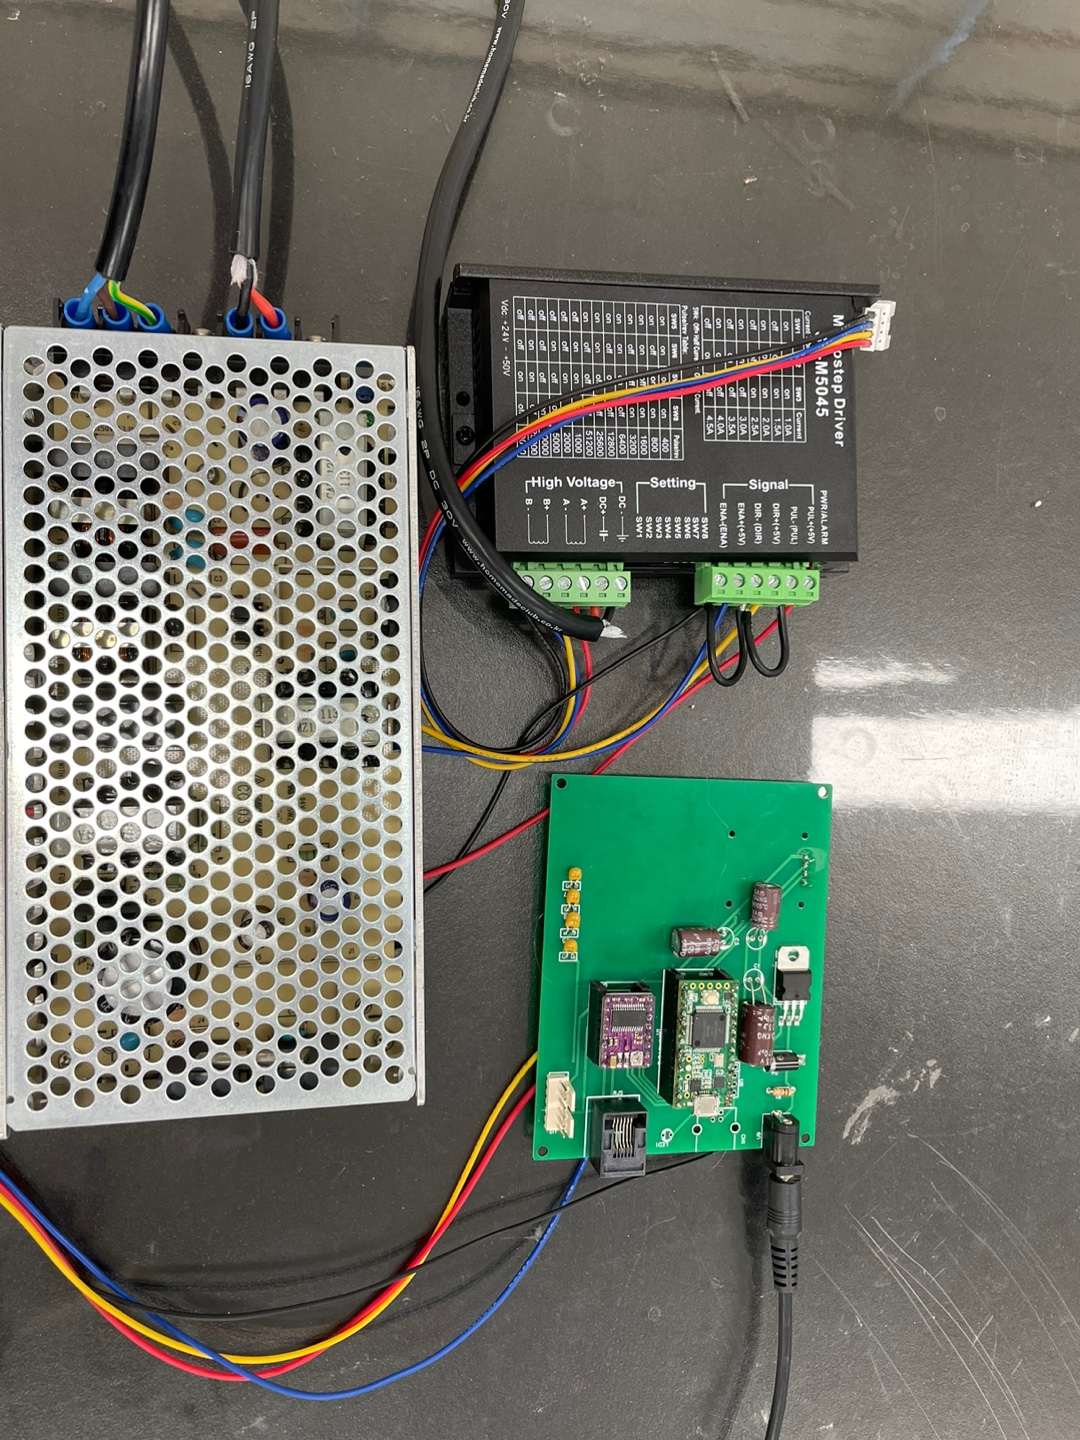
\includegraphics[clip, trim=0 100 100 100, angle=90, origin=c, width=.7\textwidth]{gdb}
		\caption{조파기 전자 회로와 모터 드라이버, 전원장치를 연결한 모습}
		\label{Wavemaker}
	\end{center}
\end{figure}


%Teensy Board 3.2, ST-M5045 스펙을 집어넣을 것.
%핀 연결은 Schematic이 있으니 굳이 따로 쓰지 말도록 하자.


% 하지만 파의 운동을 분석해보면 sin 파에 근접한 것이며 sin형으로 운동하도록 속도를 대입한 결과 판이 이상하게 운동하였다(그림 \ref{Motion of Motor}). 그리하여 제대로 sin형으로 운동할 수 있도록 다른 코드를 짰다. 조파기의 스텝 모터는 400 step 회전 시 $1~\rm{cm}$ 전진한다.

% \begin{figure}[H]
%     \centering
%     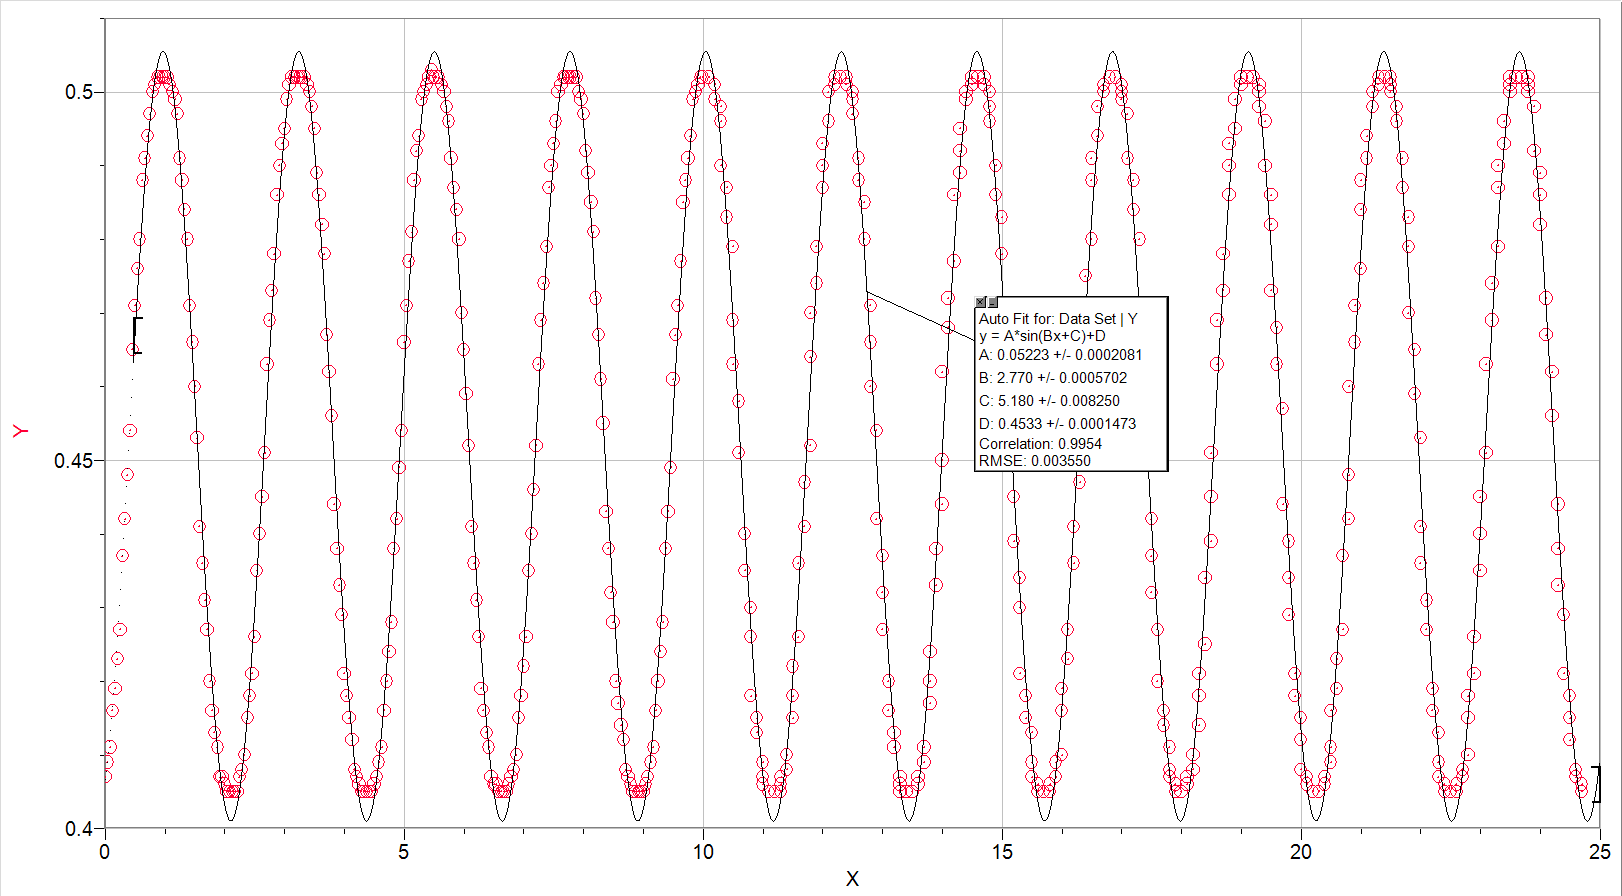
\includegraphics[height=4.5cm]{images/Linear_Motion.png}
%     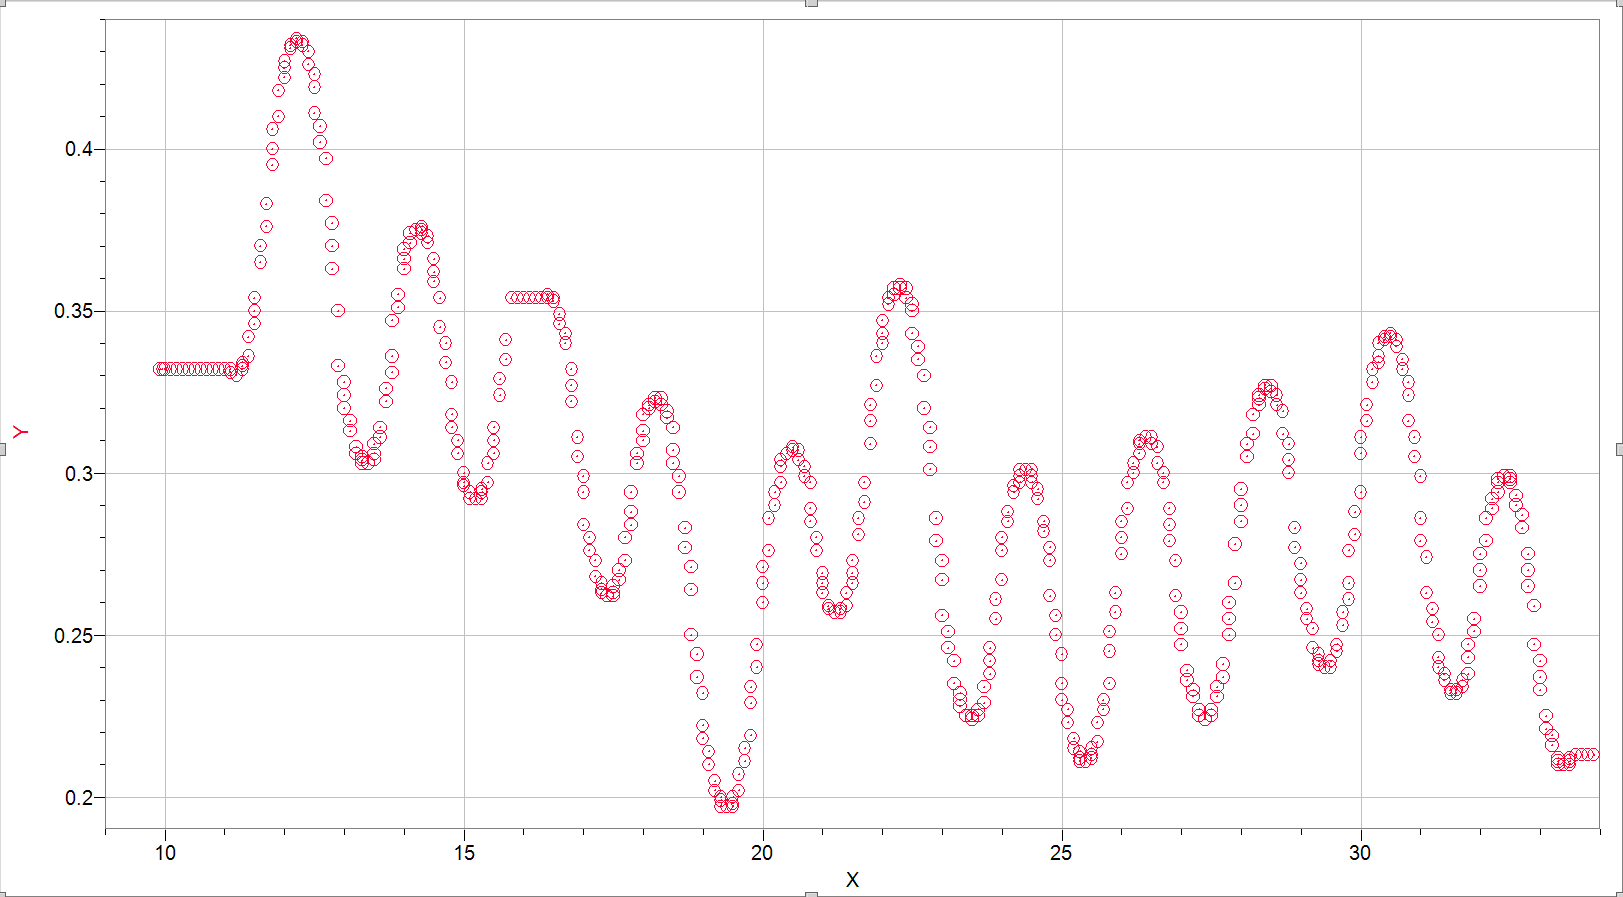
\includegraphics[height=4.5cm]{images/Sine_Motion.png}
%     \caption{모터의 선형 운동(좌)과 sin형 운동(우)}
%     \label{Motion of Motor}
% \end{figure}


\begin{figure}[H]
        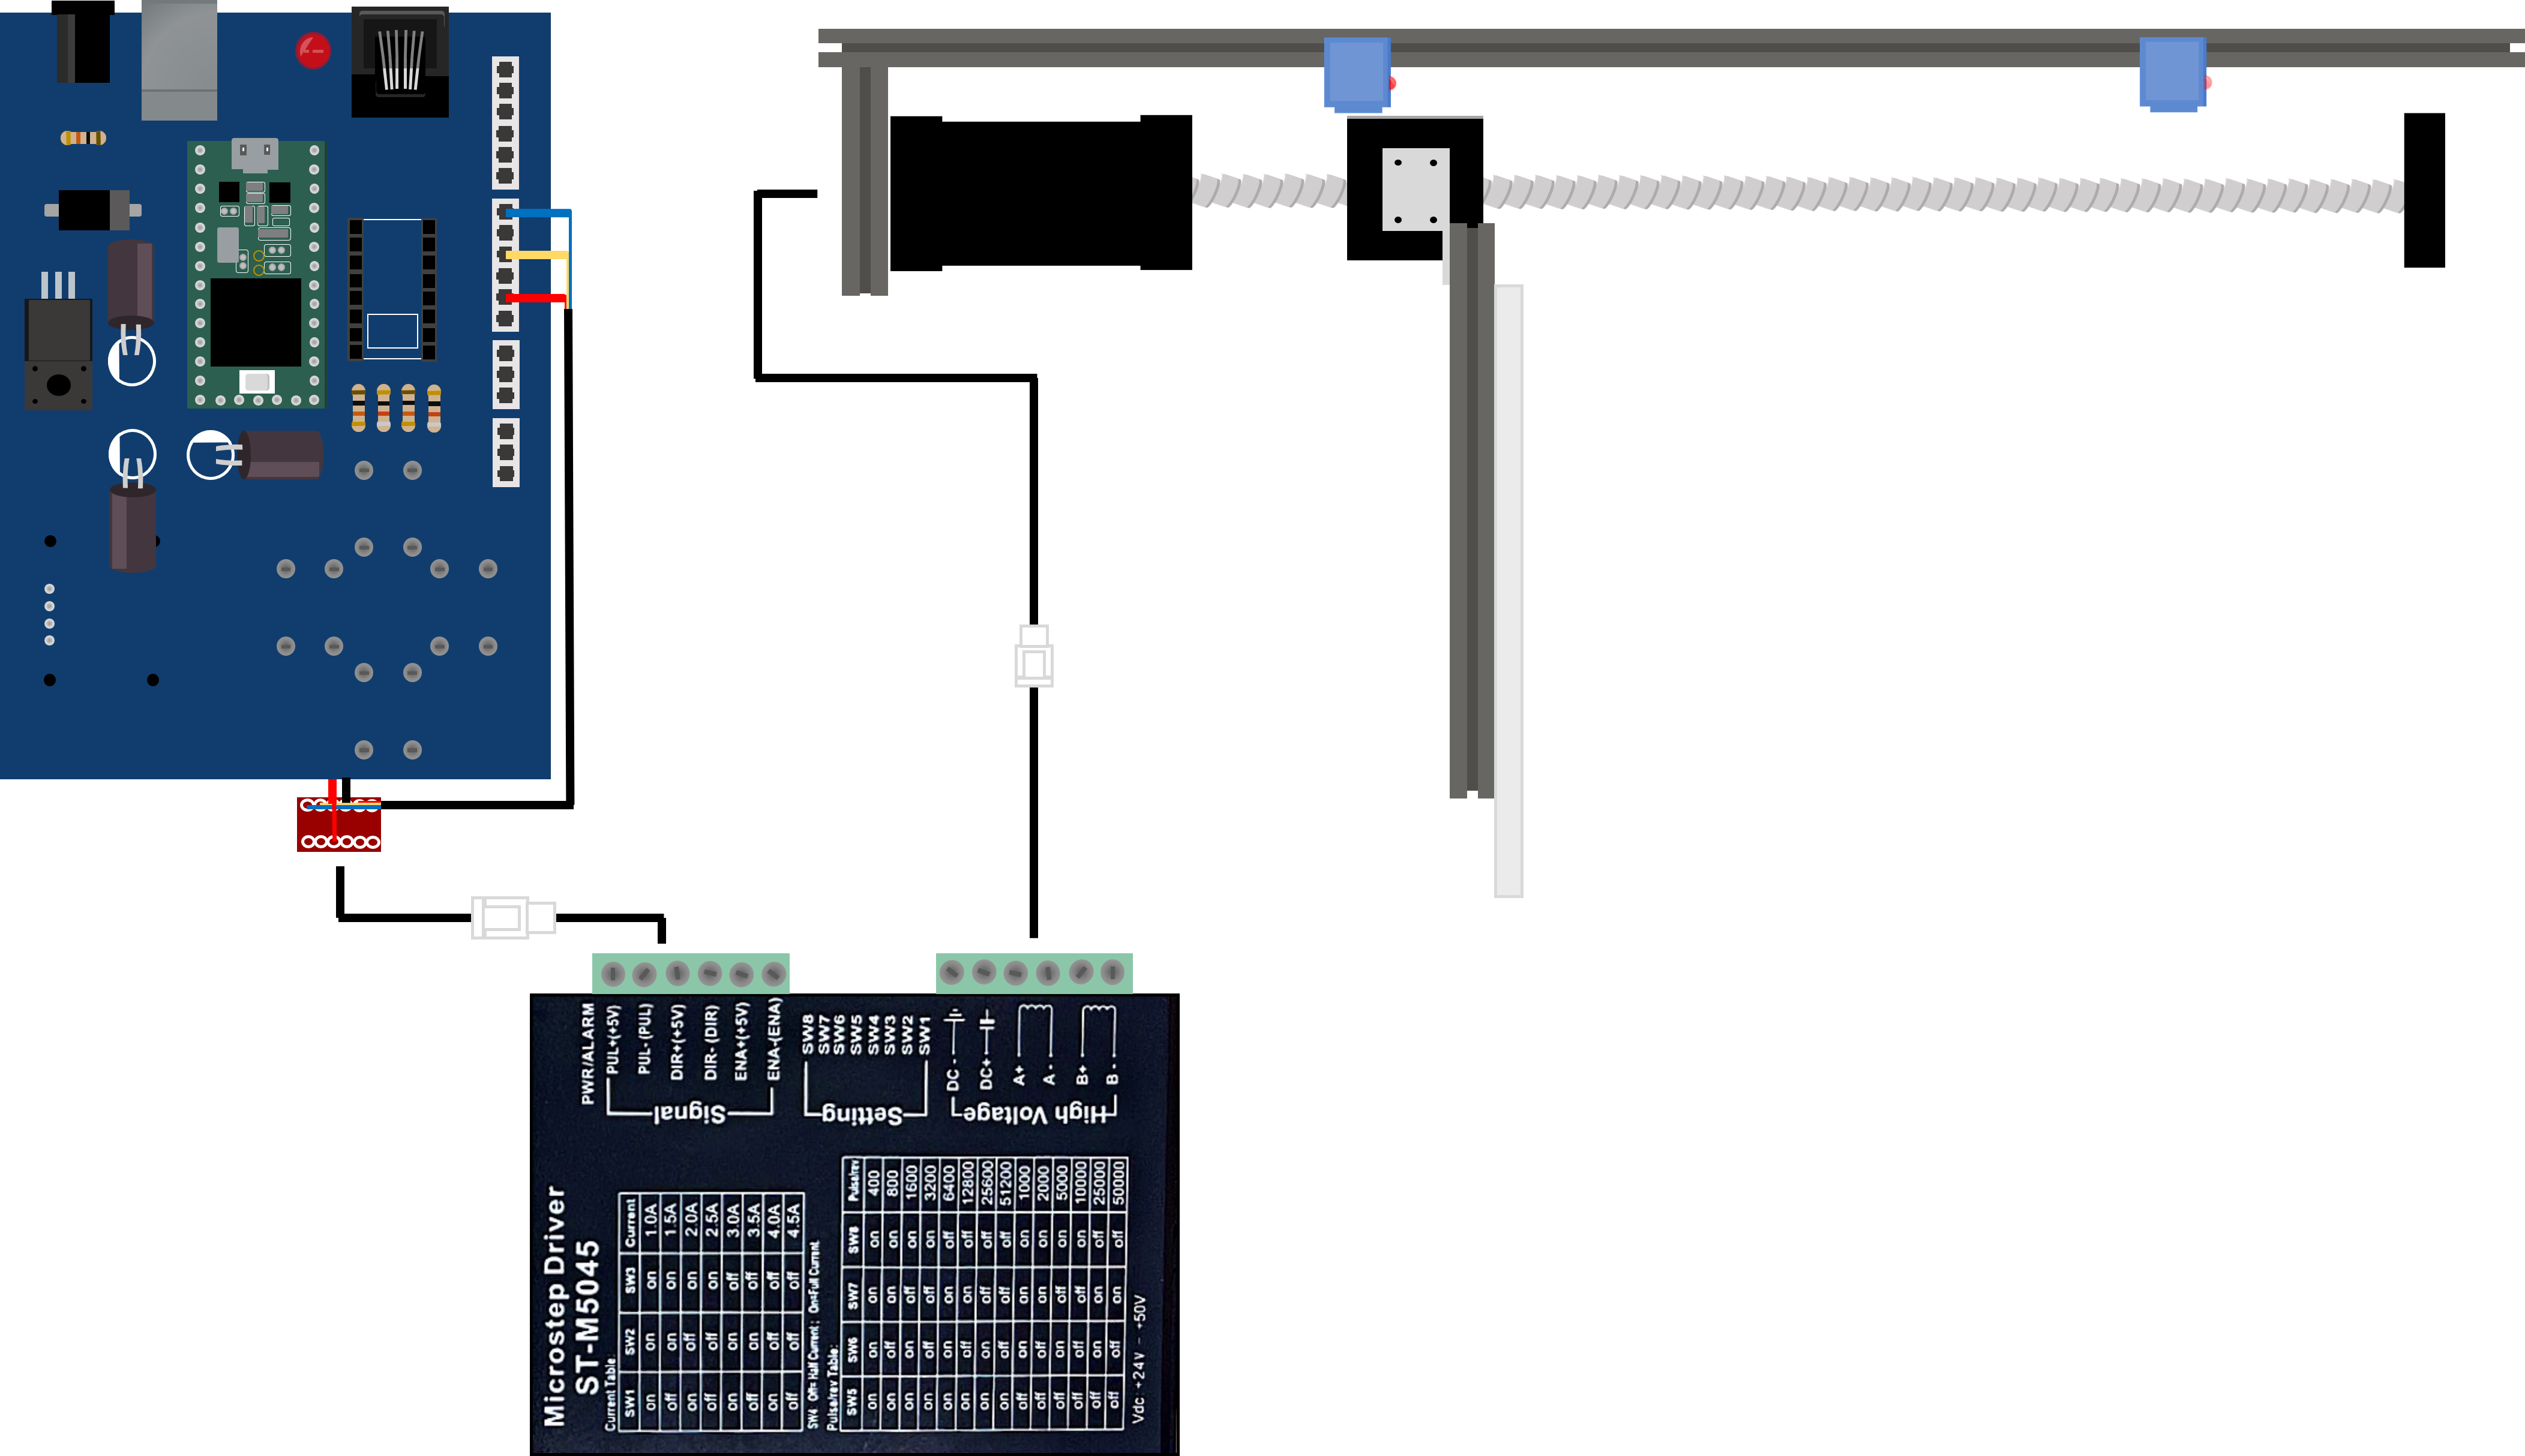
\includegraphics[width=0.9\textwidth]{images/wavemaker_control.png}
    \caption{조파기 전자 회로와 모터 드라이버, 전원장치를 연결한 모습}
    \label{wavemaker-structure}   
\end{figure}
%%%%%%%%%%%%%%%%%%%%%%%%%


\subsubsection{소프트웨어}
코딩은 Arduino를 틴지 보드에 적용할 수 있도록 컴파일러를 수정한 Teensyduino를 이용하였다. 기본적인 이동 코드는 전진, 후진이다. 스텝 모터 라이브러리는 AccelStepper, Stepper 등이 있으나 틴지 보드에서는 TeensyStep으로 모터를 더 빠르게 구동할 수 있었다. 버튼과 연계하여 각 버튼을 누를 때마다 왼쪽, 오른쪽으로 특정 변위만큼 이동하도록 할 수 있고 이를 반복하면 sin 파에 근접한 파를 만들 수 있다. 하지만 이는 근사적인 것이고 직접 변위를 대입하는 방식으로 코드를 짜서 조파기를 구동하였다.

\begin{figure}[H]
            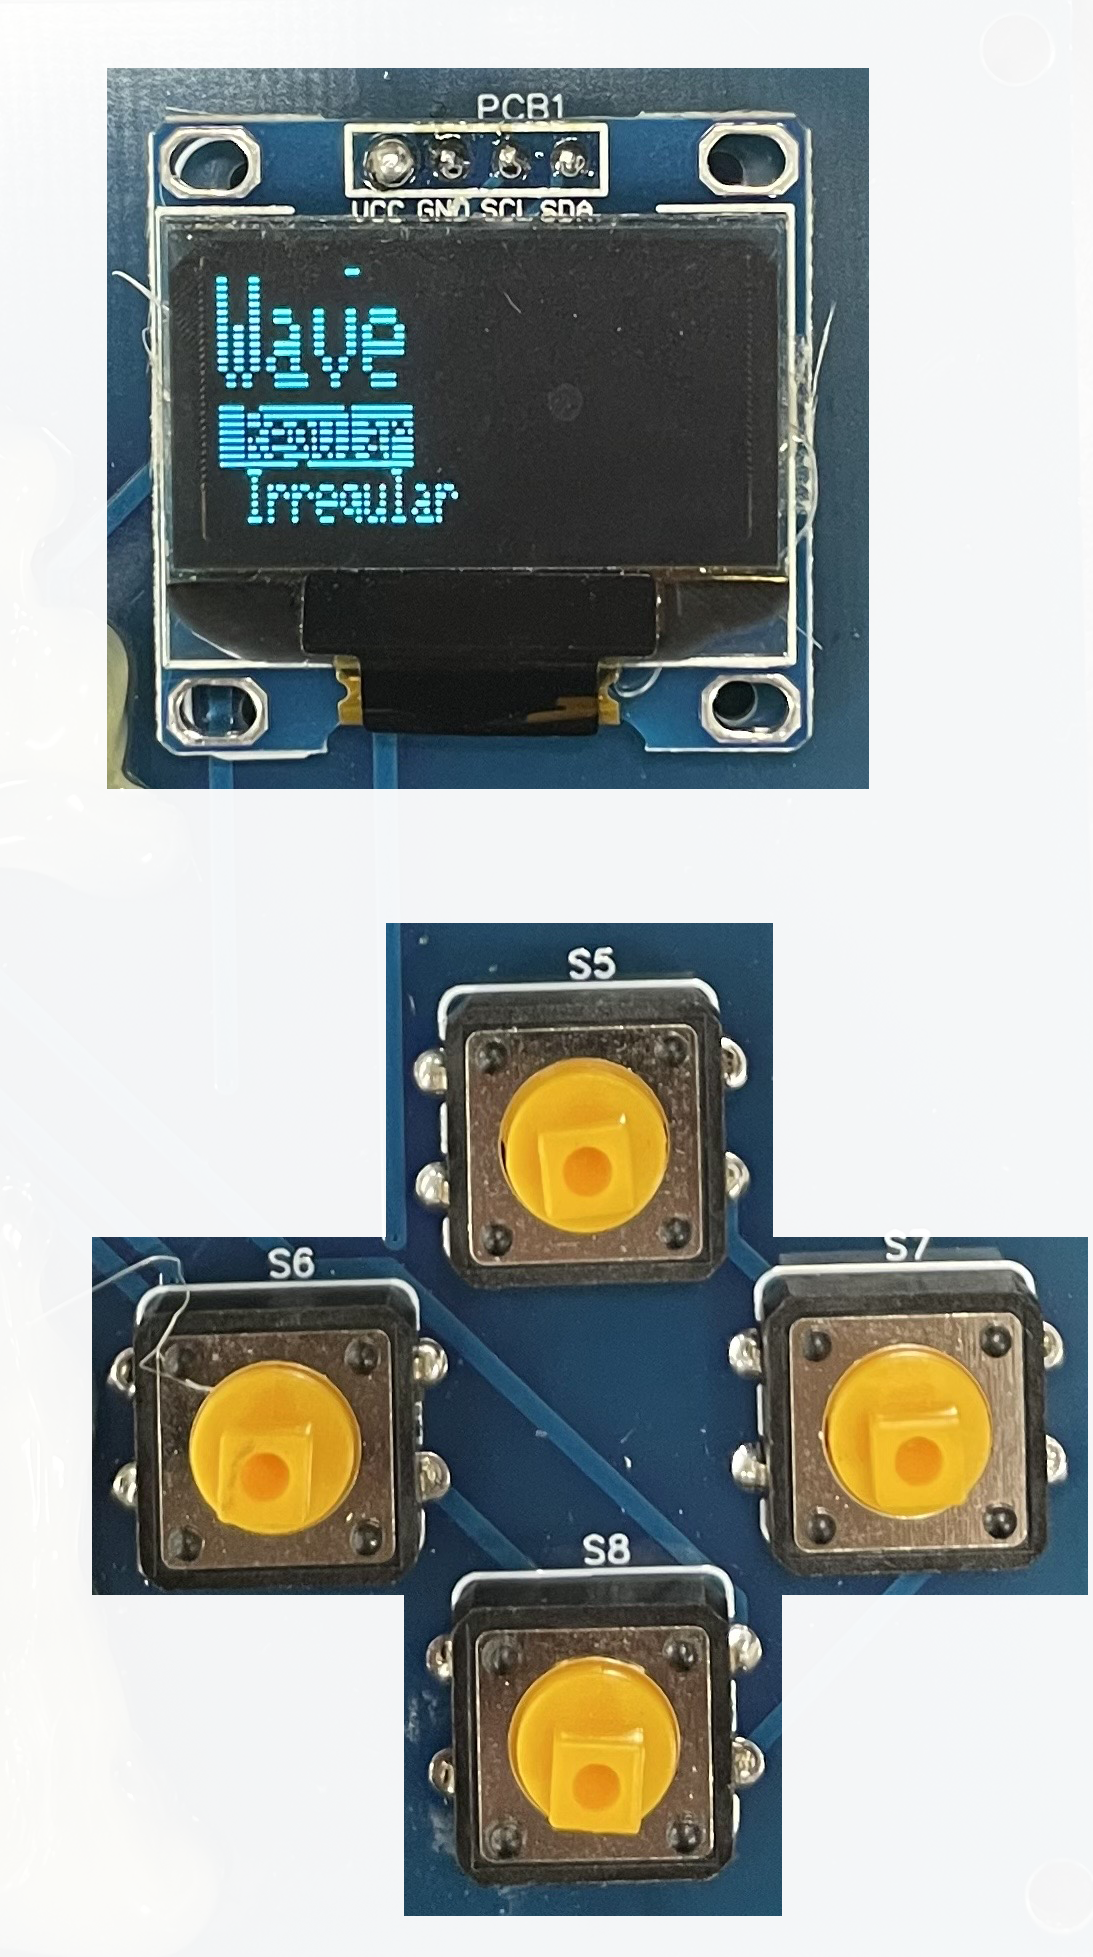
\includegraphics[trim=10 1050 100 0, clip, width=0.24\textwidth, height=3cm]{images/OLED1.png} 
            % (왼쪽, 아래(), 오른쪽, 위(숫자가 클수록 위에서 많이 잘림) )
            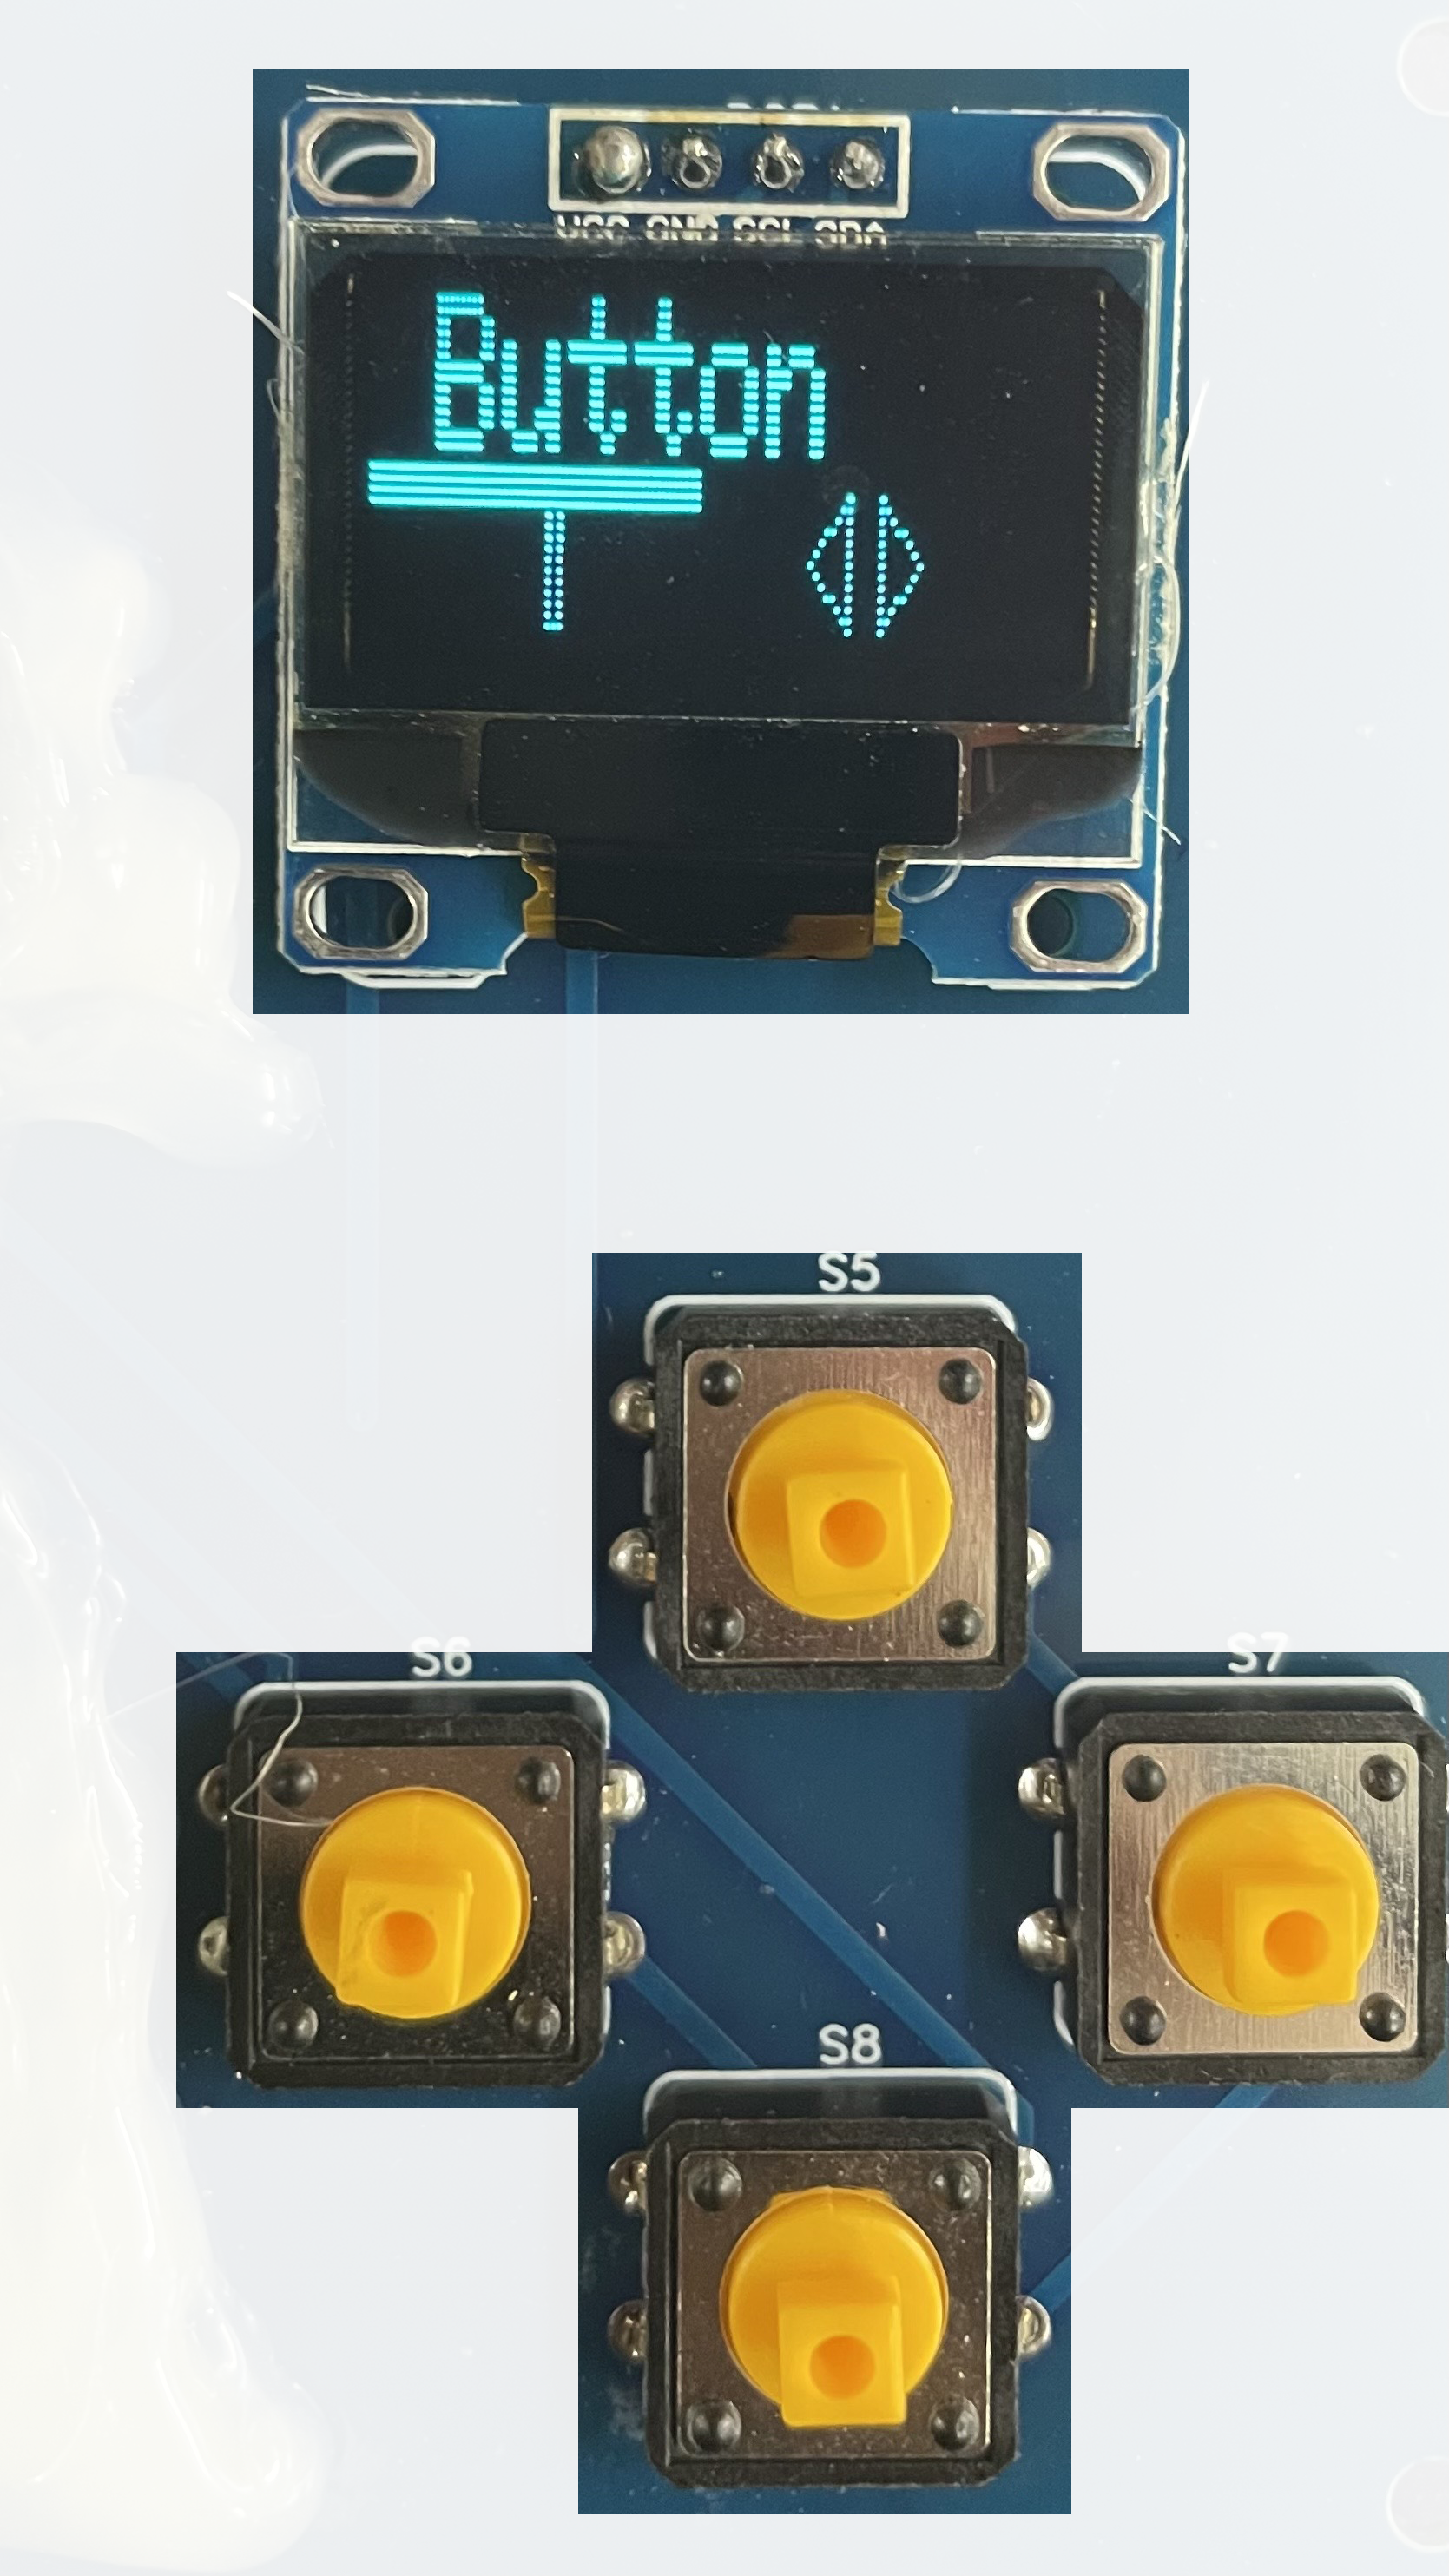
\includegraphics[trim=100 1550 100 0, clip, width=0.24\textwidth, height=3cm]{images/OLED2.png}
            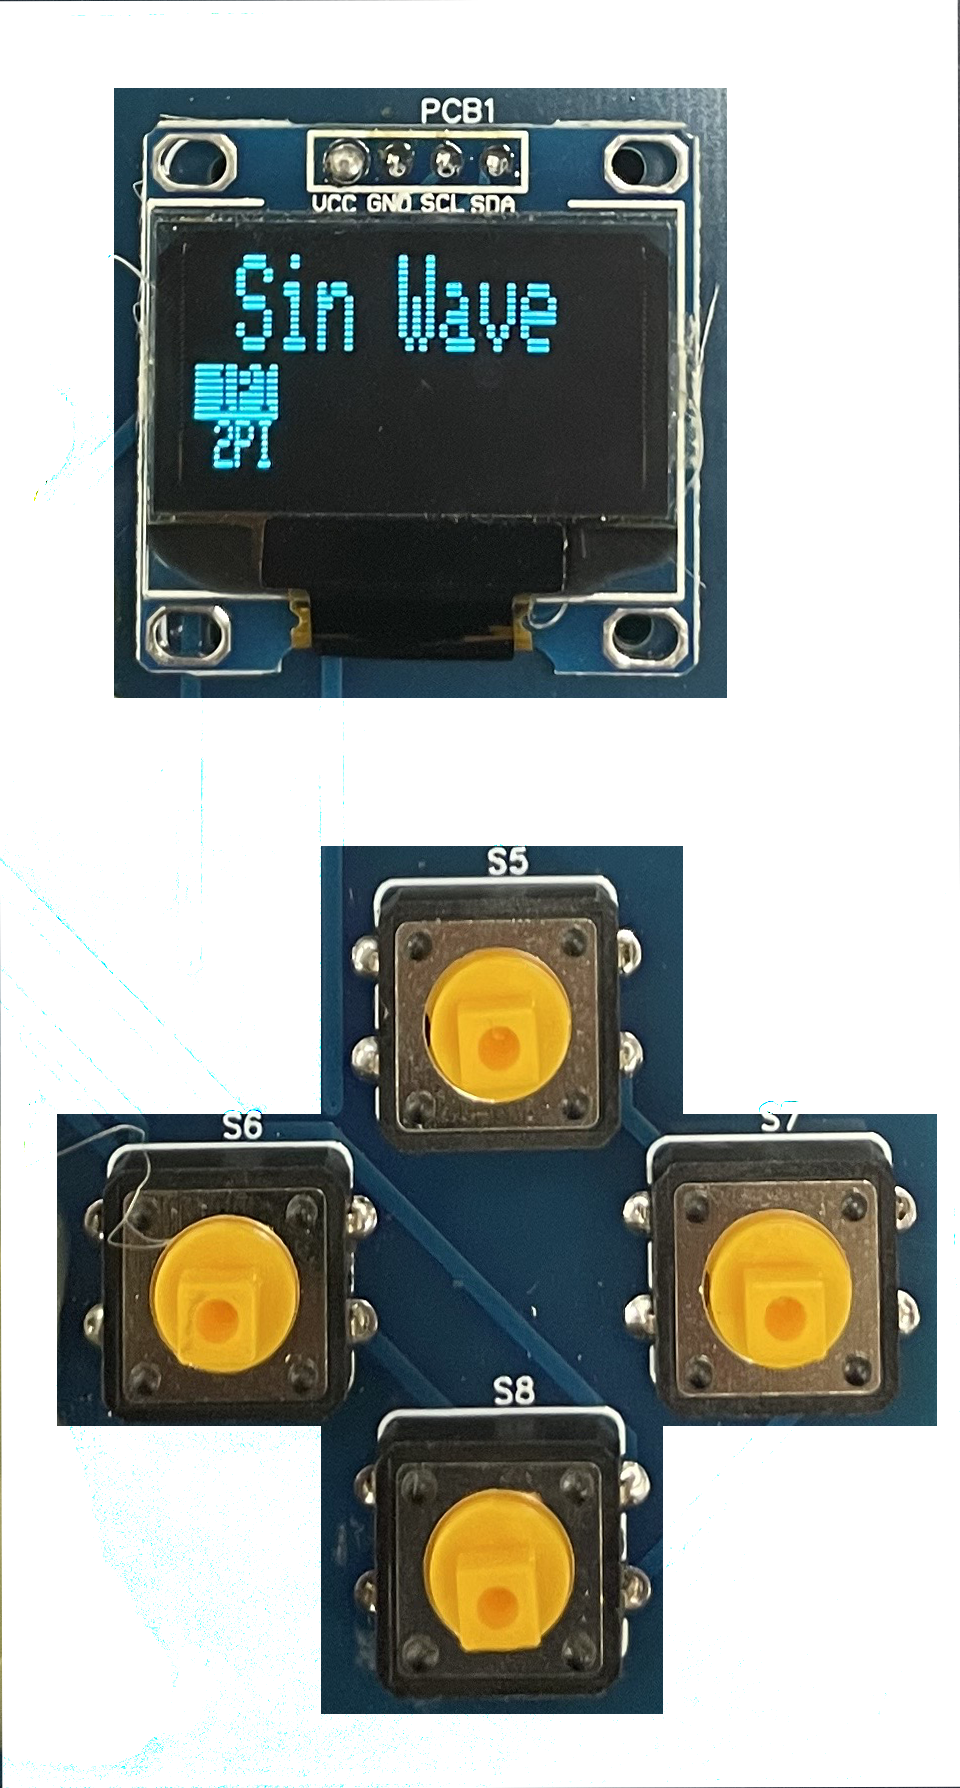
\includegraphics[trim=30 950 150 0,clip, width=0.24\textwidth, height=3cm]{images/OLED3.png}
            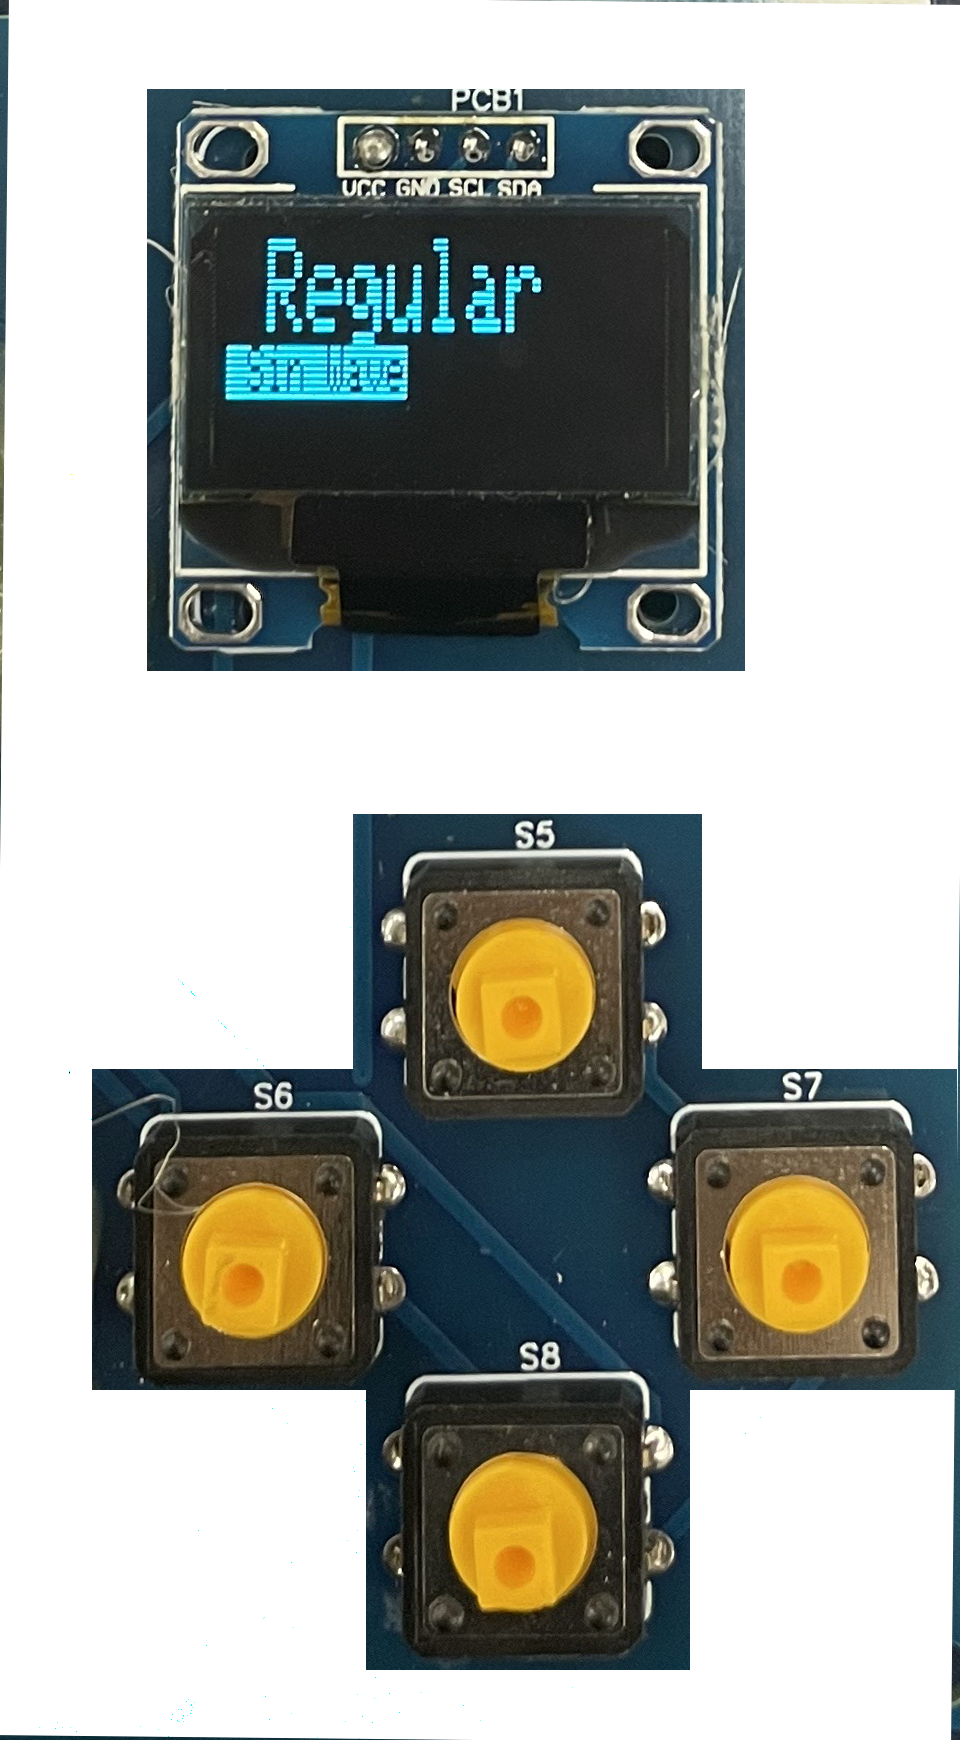
\includegraphics[trim=30 950 100 0, clip, width=0.24\textwidth, height=3cm]{images/OLED4.png}
        \caption{디스플레이 메뉴 동작 모습}
        \label{Oled}   
    \end{figure} 
    
전원을 켜면 Initialize가 실행된 후 메뉴 화면이 호출된다. 메뉴의 목록은 n진 트리의 형태로 구성되어 있으며, Wave 항목 아래에 Regular Wave, Irregular Wave, Button이 있고 각각을 버튼을 이용해 누르면 그 아래의 항목들이 호출되는 형태이다. Sin Wave의 항목에서는 변수 값을 선택해 원하는 값의 균형파를 생성할 수 있고, Button 항목에서는 원하는 방향으로 판을 움직일 수 있다.